%Document vide aux normes de l'École nationale des Chartes
%crée par J.B. Camps
%Dernières modifications E. Rouquette (03/2025)

%Personnalisation: Maëlys Gioan (2025)
% - bibliographie thématique
% - acronymes


%%%%%%%%%%%%%%%%%%%%%%%%%%%%%%%%%%%%%%%%%%%%%%%%%%%%%%%%%%%%%%%%%%
%%%%%%%%%%%%%%%%%%%%%%%%%%% PRÉAMBULE %%%%%%%%%%%%%%%%%%%%%%%%%%%%
%%%%%%%%%%%%%%%%%%%%%%%%%%%%%%%%%%%%%%%%%%%%%%%%%%%%%%%%%%%%%%%%%%


%%%%%%%%%%%%%%%%%%%%%% PARTIE OBLIGATOIRE%%%%%%%%%%%%%%%%%%%%%%%%%
%%%%%%%%%%%%%%%%%%%%%%%%%%%%%%%%%%%%%%%%%%%%%%%%%%%%%%%%%%%%%%%%%%

\documentclass[12pt,twoside]{book}
\usepackage{fontspec}
\usepackage{xunicode}
\usepackage[french]{babel}
%\setotherlanguage{} %indiquer les autres langues utilisée
\usepackage{tikz}%pour les arbres en latex intégrés au mémoire
\usetikzlibrary{mindmap,trees,positioning,shapes,arrows.meta}
\usepackage{adjustbox} %pour contrôler la taille des images et insertions


%%%%%%%%%%%%%%%%%%%%%% PARTIE OBLIGATOIRE%%%%%%%%%%%%%%%%%%%%%%%%%
%%%%%%%%%%%%%%%%%%%%%%%%%%%%%%%%%%%%%%%%%%%%%%%%%%%%%%%%%%%%%%%%%%

\usepackage{csquotes} % guillemets français
\usepackage{lettrine}

%%%%%%%%%%%%%%%%%%%%%%%%% BIBLIOGRAPHIE %%%%%%%%%%%%%%%%%%%%%%%%%%

\usepackage[style=enc,sorting=nyt,maxbibnames=10]{biblatex}% style de l'EnC (https://ctan.org/pkg/biblatex-enc)

%\defbibheading{}{\subsection*{Biblio}} % Pour changer le titre de la/les bibliographie(s)
\addbibresource{./bibliographie/archives_numeriques.bib}
\addbibresource{./bibliographie/cooperation.bib}
\addbibresource{./bibliographie/musee_air_espace.bib}
\addbibresource{./bibliographie/numerique_institution_pat.bib}
\addbibresource{./bibliographie/thesaurus.bib}
\addbibresource{./bibliographie/reflexions.bib}

%%%% Mots clés pour gérer la bibliographie thématique
\DeclareSourcemap{
	\maps[datatype=bibtex]{
		\map[overwrite]{
			\perdatasource{./bibliographie/archives_numeriques.bib}
			\step[fieldset=keywords, fieldvalue={,texArchivesNumeriques}, append]
		}
		\map[overwrite]{
			\perdatasource{./bibliographie/cooperation.bib}
			\step[fieldset=keywords, fieldvalue={,texCollab}, append]
		}
		\map[overwrite]{
			\perdatasource{./bibliographie/musee_air_espace.bib}
			\step[fieldset=keywords, fieldvalue={,texHistoire}, append]
		}
		\map[overwrite]{
			\perdatasource{./bibliographie/numerique_institution_pat.bib}
			\step[fieldset=keywords, fieldvalue={,texNumeriquePatrimoine}, append]
		}
		\map[overwrite]{
			\perdatasource{./bibliographie/thesaurus.bib}
			\step[fieldset=keywords, fieldvalue={,texThesau}, append]
		}
		\map[overwrite]{
			\perdatasource{./bibliographie/reflexions.bib}
			\step[fieldset=keywords, fieldvalue={,reflexions}, append]
		}
	}
}


%%%%%%%%%%%%%%%%%%%%%%%%%%%%% INDEX %%%%%%%%%%%%%%%%%%%%%%%%%%%%%%

\usepackage{imakeidx} %pour faire un ou plusieurs index
\makeindex %commande pour générer l'index


%%%%%%%%%%%%%%%%%%%%%%%%% ABREVIATIONS %%%%%%%%%%%%%%%%%%%%%%%%%%

\usepackage{acro}

\DeclareAcronym{mae}{short= MAE, long = Musée de l'air et de l'espace}
\DeclareAcronym{api}{short = API, long = Application Programming Interface}
\DeclareAcronym{dsc}{short = DSC, long = Département scientifique des collections}
\DeclareAcronym{drd}{short = DRD, long = Département recherche et documentation}
\DeclareAcronym{skos}{short = SKOS, long = Simple Knowledge Organization System}
\DeclareAcronym{sparql}{short = SPARQL, long = SPARQL Protocol and RDF Query Language}
\DeclareAcronym{json}{short = JSON, long = JavaScript Object Notation}
\DeclareAcronym{bnf}{short = BnF, long = Bibliothèque nationale de France}
\DeclareAcronym{siae}{short = SIAE, long = Salon international de l'aéronautique et de l'espace}
\DeclareAcronym{sigb}{short= SIGB, long = Système Intégré de Gestion de Bibliothèque}
\DeclareAcronym{cnam}{short = CNAM, long = Conservatoire National des Arts et Métiers}
\DeclareAcronym{psc}{short = PSC, long = projet scientifique et culturel}
\DeclareAcronym{anr}{short = ANR, long = Agence Nationale de la Recherche}
\DeclareAcronym{c2rmf}{short = C2RMF, long = Centre de recherche et de restauration des musées de France}

%%%%%%%%%%%%%%%%%%%%%%%%%%%%%%%%%%%%%%%%%%%%%%%%%%%%%%%%%%%%%%%%%%
%%%%%%%%%%%%%%%%%%%%%%%%% MISE EN PAGE %%%%%%%%%%%%%%%%%%%%%%%%%%%
%%%%%%%%%%%%%%%%%%%%%%%%%%%%%%%%%%%%%%%%%%%%%%%%%%%%%%%%%%%%%%%%%%


%%%%%%%%%%%%%%%%%%%%%%%%%% COMPTEURS %%%%%%%%%%%%%%%%%%%%%%%%%%%%%
%%%%%%%%%%%%%%%%%%%%%%%%%%%%%%%%%%%%%%%%%%%%%%%%%%%%%%%%%%%%%%%%%%
%%%% Sections, subsections, subsubsections

\renewcommand{\thesection}{\arabic{section}.}%On ne fait apparaître que le numéro de la section
\renewcommand{\thesubsection}{\thesection\arabic{subsection}.}%subsection en chiffres arabes
\renewcommand{\thesubsubsection}{\alph{subsubsection}.}%subsubsection en lettres minuscules
%Si l'on veut faire apparaître les subsubsection dans le table des matières (à commenter sinon)
\setcounter{tocdepth}{3}
\setcounter{secnumdepth}{3}  % La subsubsection (profondeur=3 dans la table des matières) apparait numérotée dans la TdM



%%%%%%%%%%%%%%%%%%%%%% NORMES DE L'ECOLE %%%%%%%%%%%%%%%%%%%%%%%%%
%%%%%%%%%%%%%%%%%%%%%%%%%%%%%%%%%%%%%%%%%%%%%%%%%%%%%%%%%%%%%%%%%%

\usepackage[margin=2.5cm]{geometry} %marges
\usepackage{setspace} % espacement qui permet ensuite de définir un interligne
\onehalfspacing % interligne de 1.5
\setlength\parindent{1cm} % indentation des paragraphes à 1 cm


%%%%%%%%%%%%%%%%%%%%%%%%%%% HEADERS %%%%%%%%%%%%%%%%%%%%%%%%%%%%%

\usepackage{fancyhdr} %package utilisé pour modifier les headers
\pagestyle{fancy}
\fancyhead{} % On efface tous les en-têtes existants
\fancyhead[RO]{\rightmark} % titre de chapitre à droite sur pages impaires
\fancyhead[LE]{\rightmark} % titre de chapitre à gauche sur pages paires
\setlength\headheight{16pt}%la hauteur des headers

%%%%%%%%%%%%%%%% SECTIONS dans les en-têtes %%%%%%%%%%%%%%%%%%%%%%

%%\renewcommand{\sectionmark}[1]{\markright{\small\textit{\thesection~\  #1}}}%Faire apparaître dans les headers les sections en  petit et en italiques
\renewcommand{\sectionmark}[1]{}%Commenter la ligne précédetne et mettre celle-ci pour ne pas avoir le titre des sections dans le header


%%%%%%%%%%%%%%%%%%%%%%%%% FRONTMATTER %%%%%%%%%%%%%%%%%%%%%%%%%%%%

\appto\frontmatter{\pagestyle{fancy}%
	\renewcommand{\chaptermark}[1]{\markright{\small\textit{#1}}}%
}

%%%%%%%%%%%%%%%%%%%%%%%%% MAINMATTER %%%%%%%%%%%%%%%%%%%%%%%%%%%%
\appto\mainmatter{
	\renewcommand{\chaptermark}[1]{\markright{\small\chaptername~\thechapter~--\ \textit{#1}}}%
}

%%%%%%%%%%%%%%%%%%%%%%%%%%% ANNEXES %%%%%%%%%%%%%%%%%%%%%%%%%%%%%%

\appto\appendix{
	\renewcommand{\chaptermark}[1]{\markright{\small~Annexe \thechapter~--\ \textit{#1}}}%
}


%%%%%%%%%%%%%%%%%%%%%%%%%%%%%%%%%%%%%%%%%%%%%%%%%%%%%%%%%%%%%%%%%%
%%%%%%%%%%%%%%%%%%%%%%% AUTRES PACKAGES %%%%%%%%%%%%%%%%%%%%%%%%%%
%%%%%%%%%%%%%%%%%%%%%%%%%%%%%%%%%%%%%%%%%%%%%%%%%%%%%%%%%%%%%%%%%%

%%%%%%%%%%%%%%%%%%%%%%%%%% TABLEAUX %%%%%%%%%%%%%%%%%%%%%%%%%%%%%%
%%%%%%%%%%%%%%%%%%%%%%%%%%%%%%%%%%%%%%%%%%%%%%%%%%%%%%%%%%%%%%%%%%
\usepackage{multirow}
\usepackage{ltxtable}
\usepackage{tabularx}
\usepackage{longtable}
\usepackage{booktabs}
\usepackage[table]{xcolor}
\usepackage{longtable}
\usepackage{array}
\usepackage{multirow}
\definecolor{lightgray}{gray}{0.95}

\newcolumntype{B}{>{\bfseries\raggedleft\arraybackslash}p{0.25\textwidth}}
\newcolumntype{C}{>{\raggedright\arraybackslash}p{0.75\textwidth}}
\renewcommand{\arraystretch}{1.3}  % ou 1.5 selon ton goût

%%%%%%%%%%%%%%%%%%%%%%%%% HYPHENATION %%%%%%%%%%%%%%%%%%%%%%%%%%%%
%%%%%%%%%%%%%%%%%%%%%%%%%%%%%%%%%%%%%%%%%%%%%%%%%%%%%%%%%%%%%%%%%%

%indiquer des règles d'hyphénation pour des mots précis si besoin
%\begin{hyphenrules}{french}
%	\hyphenation{}
%\end{hyphenrules}


%%%%%%%%%%%%%%%%%%%%%%%%%% HYPERREF %%%%%%%%%%%%%%%%%%%%%%%%%%%%%%
%%%%%%%%%%%%%%%%%%%%%%%%%%%%%%%%%%%%%%%%%%%%%%%%%%%%%%%%%%%%%%%%%%

% A mettre après les autres appels de packages car redéfinit certaines commandes.

\usepackage[colorlinks=false, breaklinks=true, pdfusetitle, pdfsubject ={Mémoire TNAH}, pdfkeywords={les mots-clés}]{hyperref} %
\usepackage[numbered]{bookmark}%va avec hyperref; marche mieux pour les signets. l'option numbered: les signets dans le pdf sont numérotés

% Compléter pdfsubjet et pdfkeywords
%Explication des options de hyperref (modifiables)
% hyperindex=false
% colorlinks=false: pour que le cadre des liens n'apparaisse pas à l'impression
% breaklinks permet d'avoir des liens allant sur pusieurs lignes
%pdfusetitle: utiliser \author et \title pour produire le nom et le titre du pdf


%avec overleaf, utiliser :
%\usepackage[xetex]{hyperref}
%\hypersetup{
	%	pdfauthor = {Prénom Nom},
	%	pdftitle = {titre},
	%	pdfsubject = {sujet},
	%	pdfkeywords = {premier mot-clé} {deuxième mot-clé} {troisième mot-clé} {etc}
	%}



%%%%%%%%%%%%%%%%%%%%%%%%%%%%%%%%%%%%%%%%%%%%%%%%%%%%%%%%%%%%%%%%%%
%%%%%%%%%%% COMMANDES EN ENVIRONNEMENTS PERSONNALISES %%%%%%%%%%%%
%%%%%%%%%%%%%%%%%%%%%%%%%%%%%%%%%%%%%%%%%%%%%%%%%%%%%%%%%%%%%%%%%%


%%%%%%%%%%%%%%%%%%%%%%%%%% COMMANDES %%%%%%%%%%%%%%%%%%%%%%%%%%%%%
%%%%%%%%%%%%%%%%%%%%%%%%%%%%%%%%%%%%%%%%%%%%%%%%%%%%%%%%%%%%%%%%%%
\newcommand{\mae}{\ac{mae} }

%%%%%% QUESTIONS - REPONSES pour les interviews
\newcommand{\reponse}[1]{\textbf{Réponse : }\textit{#1}}
\newcommand{\question}[1]{\textbf{Question : }#1}

%%%%%%%%%%%%%%%%%%%%%%%% ENVIRONNEMENTS %%%%%%%%%%%%%%%%%%%%%%%%%%
%%%%%%%%%%%%%%%%%%%%%%%%%%%%%%%%%%%%%%%%%%%%%%%%%%%%%%%%%%%%%%%%%%

%%%%%%%%%%%%%%%%%%%%%%%%%% GLOSSAIRE %%%%%%%%%%%%%%%%%%%%%%%%%%%%%
%%%%%%%%%%%%%%%%%%%%%%%%%%%%%%%%%%%%%%%%%%%%%%%%%%%%%%%%%%%%%%%%%%

%Exception: il faut le charger APRÈS hyperref
\usepackage[toc=false]{glossaries}
\setglossarystyle{altlistgroup}
\makeglossaries
%avec TexStudio: F9 pour compiler le glossaire (s'il y a aussi un index)

\loadglsentries{./parties/backmatter/glossaire.tex}

%%%%%%%%%%%%%%%%%%%%%%%%%%%%%%%%%%%%%%%%%%%%%%%%%%%%%%%%%%%%%%%%%%
%%%%%%%%%%%%%%% INFORMATIONS DE LA PAGE DE TITRE %%%%%%%%%%%%%%%%%
%%%%%%%%%%%%%%%%%%%%%%%%%%%%%%%%%%%%%%%%%%%%%%%%%%%%%%%%%%%%%%%%%%

\author{Maëlys \textsc{Gioan} - M2 TNAH}
\title{Gestion de l'information à l'ère du numérique : entre héritage et innovation}


%%%%%%%%%%%%%%%%%%%%%%%%%%%%%%%%%%%%%%%%%%%%%%%%%%%%%%%%%%%%%%%%%%
%%%%%%%%%%%%%%%%%%%%%%%%%%%%%%%%%%%%%%%%%%%%%%%%%%%%%%%%%%%%%%%%%%
%%%%%%%%%%%%%%%%%%%%%%%%%% DOCUMENT %%%%%%%%%%%%%%%%%%%%%%%%%%%%%%
%%%%%%%%%%%%%%%%%%%%%%%%%%%%%%%%%%%%%%%%%%%%%%%%%%%%%%%%%%%%%%%%%%
%%%%%%%%%%%%%%%%%%%%%%%%%%%%%%%%%%%%%%%%%%%%%%%%%%%%%%%%%%%%%%%%%%



\begin{document}
	
	%%%%%%%%%%%%%%%%%%%%%%%%%%%%%%%%%%%%%%%%%%%%%%%%%%%%%%%%%%%%%%%%%%
	%%%%%%%%%%%%%%%%%%%%%%%%% FRONTMATTER %%%%%%%%%%%%%%%%%%%%%%%%%%%%
	%%%%%%%%%%%%%%%%%%%%%%%%%%%%%%%%%%%%%%%%%%%%%%%%%%%%%%%%%%%%%%%%%%
	
	%%%%%%%%%%%%%%%%%%%%%%%%% PAGE DE TITRE %%%%%%%%%%%%%%%%%%%%%%%%%%
	%%%%%%%%%%%%%%%%%%%%%%%%%%%%%%%%%%%%%%%%%%%%%%%%%%%%%%%%%%%%%%%%%%
	
	\begin{titlepage}
		\begin{center}
			
			\bigskip
			
			\begin{large}				
				ÉCOLE NATIONALE DES CHARTES\\
				UNIVERSITÉ PARIS, SCIENCES \& LETTRES
			\end{large}
			\begin{center}\rule{2cm}{0.02cm}\end{center}
			
			\bigskip
			\bigskip
			\bigskip
			\begin{Large}
				\textbf{Maëlys Gioan}\\
			\end{Large}
			%selon le cas
			\begin{normalsize} \textit{licenciée ès histoire}\\
				%\textit{diplômé.e de master}
			\end{normalsize}
			
			\bigskip
			\bigskip
			\bigskip
			
			\begin{Huge}
				\MakeUppercase{\textbf{La gestion de l'information à l'ère du numérique.\\ \textit{Entre héritage et innovation}}}\\
			\end{Huge}
			\bigskip
			\bigskip
			\begin{LARGE}
				\textbf{Le cas du Musée de l'Air et de l'Espace}\\
			\end{LARGE}
			
			\bigskip
			\bigskip
			\bigskip
			\begin{large}
			\end{large}
			\vfill
			
			\begin{large}
				Mémoire pour le diplôme de master \\
				\enquote{Technologies numériques appliquées à l'histoire} \\
				\bigskip
				2025
			\end{large}
			
		\end{center}
	\end{titlepage}
	
	\thispagestyle{empty}	
	\cleardoublepage
	
	\frontmatter
	
	
	%%%%%%%%%%%%%%%%%%%%%%%%%%%% RESUME %%%%%%%%%%%%%%%%%%%%%%%%%%%%%%
	%%%%%%%%%%%%%%%%%%%%%%%%%%%%%%%%%%%%%%%%%%%%%%%%%%%%%%%%%%%%%%%%%%
	
	
	\chapter{Résumé}
	\medskip
	Résumé du mémoire en français. Cette page ne doit pas dépasser une page.\\
	
	\textbf{Mots-clés:} une liste de mots-clés~; séparés par des points-virgules.
	
	\textbf{Informations bibliographiques:} GIOAN Maëlys, \textit{Gestion de l'information à l'ère du numérique : entre héritage et innovation. Le cas du Musée de l'Air et de l'Espace}, mémoire de master \enquote{Technologies numériques appliquées à l'histoire}, dir. Emmanuelle Bermès, Valérie Joyaux, École nationale des chartes, 2025.
	
	\newpage{\pagestyle{empty}\cleardoublepage}
	
	%%%%%%%%%%%%%%%%%%%%%%%%% REMERCIEMENTS %%%%%%%%%%%%%%%%%%%%%%%%%%
	%%%%%%%%%%%%%%%%%%%%%%%%%%%%%%%%%%%%%%%%%%%%%%%%%%%%%%%%%%%%%%%%%%
	
	\chapter{Remerciements}
	
	\lettrine{M}es remerciements vont tout d'abord à\dots
	\newpage{\pagestyle{empty}\cleardoublepage}
	
	\chapter{Liste des abréviations}
	\printacronyms[heading=none]
	
	%%%%%%%%%%%%%%%%%%%%%%%%% BIBLIOGRAPHIE %%%%%%%%%%%%%%%%%%%%%%%%%%
	%%%%%%%%%%%%%%%%%%%%%%%%%%%%%%%%%%%%%%%%%%%%%%%%%%%%%%%%%%%%%%%%%%
	
	\chapter{Bibliographie}
	%\addcontentsline{toc}{chapter}{Bibliographie}
	\printbibliography[keyword={texHistoire}, title={Histoire du musée de l'air et de l'espace}]
	\printbibliography[keyword={texCollab}, title={Collaboration entre institutions patrimoniales}]
	\printbibliography[keyword={texNumeriquePatrimoine}, title={Numérique en institution patrimoniale}]
	\printbibliography[keyword={texArchivesNumeriques}, title={Archives Numériques}]
	\printbibliography[keyword={texThesau}, title={Gestion de thésaurus}]
	\printbibliography[keyword={reflexions}, title={Références littéraires}]
	
	
	
	%%%%%%%%%%%%%%%%%%%%%%%%% INTRODUCTION %%%%%%%%%%%%%%%%%%%%%%%%%%%
	%%%%%%%%%%%%%%%%%%%%%%%%%%%%%%%%%%%%%%%%%%%%%%%%%%%%%%%%%%%%%%%%%%
	
	% Pour intégrer l'ensemble de la biblio au début
	\nocite{*}
	
	\chapter{Introduction}	

\begin{quote}
    \og La Bibliothèque comporte toutes les structures verbales, toutes les variations que permettent les vingt-cinq symboles orthographiques, mais point un seul non-sens absolu [...] Je ne puis combiner une série quelconque de caractères, par exemple	\textit{Dhcmrlchtdj} que la divine Bibliothèque n’ait déjà prévue, et qui dans quelqu'une de ses langues secrètes ne renferme
	une signification terrible\footcite{borgesBibliothequeBabel1963}.\fg
\end{quote} %Input: importer un fichier
	
	\newpage{\pagestyle{empty}\cleardoublepage}
	
	%%%%%%%%%%%%%%%%%%%%%%%%%%%%%%%%%%%%%%%%%%%%%%%%%%%%%%%%%%%%%%%%%%
	%%%%%%%%%%%%%%%%%%%%%%%%% MAINMATTER %%%%%%%%%%%%%%%%%%%%%%%%%%%%%
	%%%%%%%%%%%%%%%%%%%%%%%%%%%%%%%%%%%%%%%%%%%%%%%%%%%%%%%%%%%%%%%%%%
	
	\mainmatter
	
	%%%%%%%%%%%%%%%%%%%%%%%%%%% PARTIE I %%%%%%%%%%%%%%%%%%%%%%%%%%%%%
	%%%%%%%%%%%%%%%%%%%%%%%%%%%%%%%%%%%%%%%%%%%%%%%%%%%%%%%%%%%%%%%%%%
	
	\part{Le contexte institutionnel particulier du Musée de l'air et de l'espace}
	
	%%%%%%%%%%%%%%%%%%%%%%%%%% INTRODUCTION %%%%%%%%%%%%%%%%%%%%%%%%%%
	
	Ici, je pourrai mettre une introduction de ma première partie.
	
	%%%%%%%%%%%%%%%%%%%%%%%%%%%%% TEXTE %%%%%%%%%%%%%%%%%%%%%%%%%%%%%
	
	\chapter[Une référence nationale]{\label{I-A}Le \mae : une référence nationale pour les collections aéronautiques}

\lettrine{L}e \maelong~du Bourget occupe une position singulière dans le paysage muséographique français. Cette institution aux collections exceptionnelles incarne nombre des défis contemporains de la conservation patrimoniale appliquée aux objets technologiques. Cette histoire mouvementée en fait une institution unique qui témoigne des difficultés rencontrées par les institutions dédiées au patrimoine technique pour trouver leur légitimité, elle a également façonné un musée unique qui dépasse la simple fonction de conservatoire pour s'affirmer comme un acteur de la recherche aéronautique.

\section{\label{I-A-1}La représentation nationale : un musée aux collections uniques}

\subsection{La lente construction du \mae}

L'histoire du \acf{mae}\footnote{Voir la chronologie de l'histoire du musée en annexe \ref{Ax-A}.} est celle d'un projet persistant, sans cesse reporté et modifié, qui trouve ses racines dès la fin du XIXe siècle dans les aspirations d'associations ou de personnalités liées à l'aéronautique\footcite{terrierAeroportParisBourget2019}. Aujourd'hui encore, il ne cesse d'évoluer : l'année 2025 a ainsi vu, en plus des modernisations logicielles majeures, l'inauguration d'un nouvel espace d'exposition permanente valorisant la tour de contrôle de l'aéroport historique du Bourget\footcite{museedelairetdelespaceHallNavigationAerienne2025}. C'est en effet dans ces locaux que le musée s'est installé en 1973, après une longue période de recherches pour une implantation pérenne. Confronté aux aléas du XXe siècle, aux contraintes de conservation d'objets techniques et aux hésitations ministérielles, le projet d'installation doit sa concrétisation à l'engagement de militaires, de passionnés et au poids de sa mission de vitrine d'un savoir-faire français.

La décision devient effective après la Première Guerre mondiale, premier conflit à exploiter l'importance stratégique de l'aviation. À l'initiative d'Albert Caquot, un conservatoire de l'aéronautique est confié au capitaine Hirschauer : quelques aéronefs trouvent refuge à Issy-les-Moulineaux, avant d'être déplacés à Chalais-Meudon à la suite d'une crue de la Seine. Le musée est officiellement inauguré le 23 novembre 1921 : l'institution naît, mais sans réel ancrage territorial. Pendant l'entre-deux-guerres, d'autres implantations sont tentées, notamment boulevard Victor à Paris. Ces locaux ouverts en 1936 ferment trois ans plus tard à l'aube de la Seconde Guerre mondiale. Bombardements et saisies allemandes interrompent son élan ; à la Libération, le musée réintègre Chalais-Meudon, mais demeure fermé au public durant plus de quinze ans.

S'ensuit une longue période d'incertitudes : entre 1952 et 1972, vingt-et-un sites sont envisagés\footcite{terrierAeroportParisBourget2019}. En 1961, le musée rouvre à Meudon, mais provisoirement. Le « Palais de l'Air » poursuit sa quête de locaux adaptés à la monumentalité de ses collections. En 1973, l'ancien aéroport du Bourget, libéré au profit d'Orly, est retenu comme implantation définitive.

Dès son ouverture, le musée affirme un lien fort avec l’État et l’industrie aéronautique : le prototype Concorde 001 lui est offert par l'état français à l'occasion de son inauguration. Les collections sont progressivement transférées, Chalais-Meudon ferme en 1981, la direction rejoint le Bourget, de nouveaux halls sont ouverts au fil de l’extension du site. C'est avec l'ouverture d'un hall dédié à l'espace en 1983 que le musée prend son nom actuel : \acf{mae}.

Cette consolidation s’accompagne de son intégration à un réseau de musées techniques et de l'armée, et à d'importants chantiers de modernisation : un Planétarium est ouvert en 1985, de nouvelles réserves sont installées à Dugny, l'informatisation des métiers du musée s'amorce dès les années 1990 avec la mise en place de \gls{micromusee} pour les collections, et du \ac{sigb} \gls{alexandrie} pour la bibliothèque. En 2016, l’e-médiathèque est lancée pour gérer les fonds audiovisuels. Cette professionnalisation du musée est notamment marquée en 2002 par sa labellisation \enquote{Musée de France}. Ce mouvement ce poursuit aujourd’hui : les outils de gestion des collections du musées et de la bibliothèque ont été renouvelés définitivement en juillet 2025, de nouveaux espaces de conservation et d’exposition sont en projet, et l'intégration du musée au réseau du Grand Paris Express laisse espérer un surcroît de fréquentation.

Né tout d'abord de ses collections et non d'un site, le \mae, dédié à la mémoire du ciel, est aujourd'hui devenu indissociable de ses locaux emblématiques de l'aéronautique française pour devenir une un musée incontournable.

\subsection{Une institution complexe qui fait référence}

C’est à partir des années 1980 que le musée se structure véritablement, sous l’effet conjoint d’une reconnaissance de l’importance culturelle de l’aéronautique, d’un renouveau muséographique et de son inscription dans les réseaux nationaux. 
Son installation dans les locaux de l'ancien aéroport du Bourget incarne sa double fonction : conservatoire historique de l'aéronautique française, et vitrine stratégique d'un secteur en plein développement. Premier aérodrome civil parisien\footcite{terrierAeroportParisBourget2019}, ce lieu symbolique ancre en effet le musée dans la géographie et l’histoire de l’aviation française. Son lien avec le \ac{siae}, qu’il accueille tous les deux ans, renforce sa fonction de représentation.
La multiplicité des missions du \mae est parfaitement soulignée par Clémence Raynaud dans un article sur les collections iconographiques du \mae : tout d'abord dédié à la documentation de l'histoire et des techniques de l'aéronautique, le musée s'est développé \enquote{comme un établissement à vocation universelle embrassant de multiples aspects du fait aérien, que l’étiquette technique caractérise aujourd’hui d’une manière partielle\footcite{raynaudMuseeTechniqueDhistoire2018}.} Selon l'auteur, qui cite le \ac{psc} 2007, c'est autour des années 2010 que le musée s'affirme comme un \enquote{musée technique, d’histoire et de société}.

C'est là en effet l'un des grands défis auxquels il est confronté : le \mae possède des collections très riches et hétérogènes, sans équivalent national. On y trouve des aéronefs, moteurs, équipements techniques — objets exigeant des conditions de conservation particulières et une expertise rare. Cette spécificité impose des pratiques adaptées et des vocabulaires spécialisés. Mais le musée ne s’y limite pas : maquettes, estampes, objets d’art, uniformes, et, plus récemment, objets civils — vêtements, vaisselle, jouets — reflètent une évolution vers une muséographie anthropologique. Cette inflexion est incarnée notamment par la création d'un département des collections artistiques et anthropologiques, et la diversité des objets conservés se retrouve dans le schéma ci-dessous qui rassemble les différents noms de domaines des collections du musée.

\begin{figure}[htbp]
	\centering
	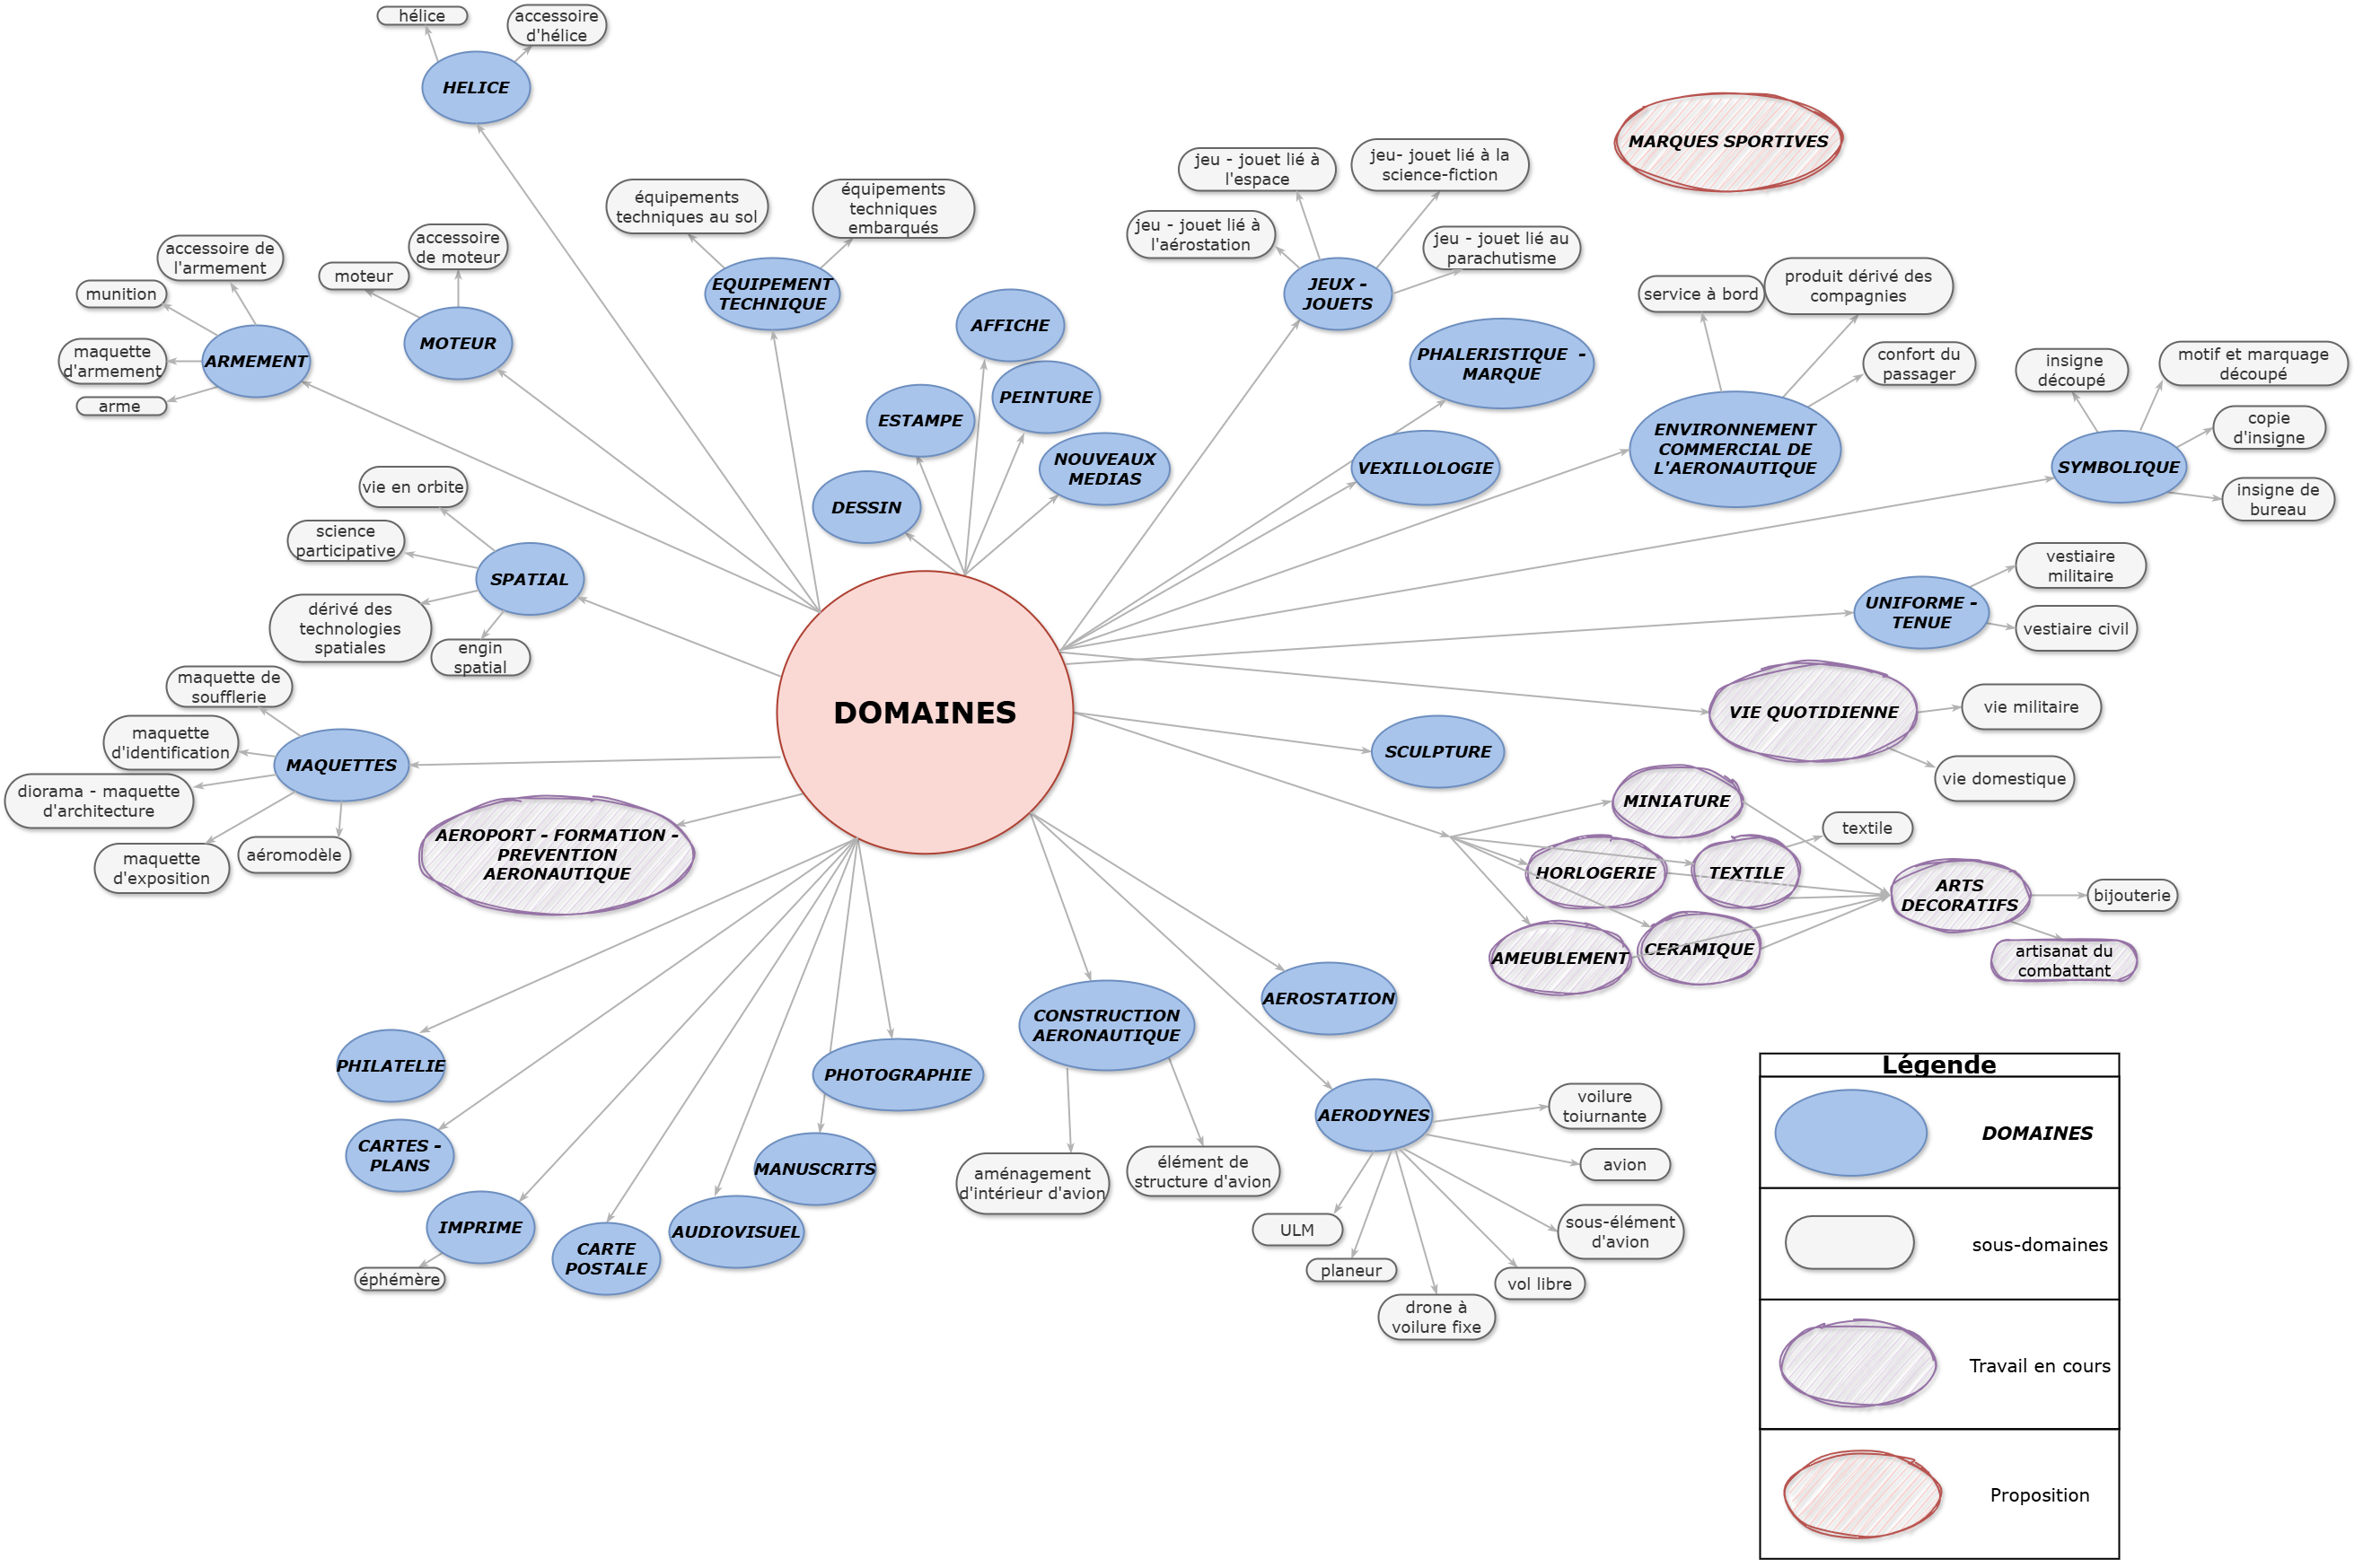
\includegraphics[width=\linewidth]{img/MODEL_domaines.png}
	\caption{Modélisation du thésaurus des domaines utilisés par le \mae}
	\label{fig:model_domaines}
\end{figure}

Le \mae incarne donc des défis propres aux musées techniques, bien différents de ceux des musées de beaux-arts et qui imposent des compétences croisées à la fois techniques et muséales. Les jeunes chargés de collections sont ainsi souvent issus de formations spécialisés — comme les masters du Muséum d’histoire naturelle — et passent par des institutions techniques ou militaires, telles que le musée de la Marine, le musée de l’Armée ou le \ac{cnam}. Ces musées doivent sans cesse composer avec des objets singuliers, souvent massifs, complexes à restaurer et à exposer.

Ces multiples défis sont rappelés par Agnès Mirambet-Paris et François Mirambet : diversité des matériaux, état de dégradation, inadéquation des environnements de conservation, échelle des objets, lourdeur des procédures, et besoin de ressources spécialisées\footcite{mirambet-parisConservationrestaurationPatrimoineTechnique2011}. Ils insistent sur la nécessité du dialogue entre techniciens et restaurateurs :
\begin{quote}
	\og C’est bien par le partage de compétences techniques acquises dans le domaine industriel et celles obtenues dans les écoles de formation à la restauration que pourront se développer pleinement des travaux de restauration\footcite{mirambet-parisConservationrestaurationPatrimoineTechnique2011}.\fg
\end{quote}

Le \mae incarne cette articulation entre expertise technique et exigence muséale. Ses pièces emblématiques — comme le Concorde 001 ou le scaphandre de Jean-Loup Chrétien\footcite{champenoisTresorsMuseeLair} — en font une institution unique, au croisement des enjeux de représentation nationale, de préservation patrimoniale et d’innovation culturelle.


\section{\label{I-A-2}La recherche : le rôle déterminant d'un musée technique}

Le rôle du \ac{mae} ne se cantonne pas seulement à la seule conservation d’objets : celui-ci s'impose en effet comme un acteur essentiel de la recherche au carrefour entre histoire technique, aéronautique, sciences sociales et muséologie.  Le \ac{psc} du \acf{mae}, remanié en 2020, est un précieux témoin du difficile équilibre recherché par le musée pour assurer la visibilité et valorisation de ses fonds auprès du grand public comme de la communauté scientifique.

\subsection{Un acteur central dans les réseaux de recherche aéronautique}

Le \ac{mae} se retrouve en effet, comme bien des musées techniques ou beaux-arts, pris entre différents mondes : musées, bibliothèques, archives, centres de recherches, associations de passionnés... Une grande partie de sa mission consiste donc à assurer la communication entre ces différents qui échangent savoir, pratiques et innovations dans un réseau national comme international.

Ce rôle se manifeste dans la multiplication des expositions temporaires à dimension internationale : l’exposition \emph{Flight}, fruit d’un partenariat avec le Parque de las Ciencias de Grenade, le centre Techmania de Plzeň et l’Institut royal des Sciences naturelles de Belgique, illustre ainsi la capacité du musée à fédérer des acteurs divers autour d’une réflexion sur le vol humain et animal\footnote{Voir \href{https://www.museeairespace.fr/agenda/exposition-flight}{https://www.museeairespace.fr/agenda/exposition-flight}}. De même, des journées d’études, comme celle organisée en 2019 pour le centenaire de l’aviation civile\footnote{Programme disponible sur le site du musée \cite{19192019CentAns}}, réunissent des universitaires, des conservateurs, des ingénieurs ou des amateurs, se retrouvant pour croiser les regards et les méthodes pour améliorer notre compréhension de l'histoire ou encore de la sociologie de l'aéronautique.

L’engagement du musée ne s’arrête pas à la diffusion : il participe à des projets de recherche interdisciplinaires comme le programme C-ADER déposé auprès de l'\ac{anr}, et qui fédère le \ac{c2rmf}, l’Institut de recherche de chimie Paris, l’université de Lorraine et l’Institut de soudure, autour de la  question de la conservation des aéronefs exposés en extérieur\footnote{Voir  \href{https://anr.fr/Projet-ANR-22-CE27-0025}{https://anr.fr/Projet-ANR-22-CE27-0025}}. Ce projet transversal conduira entre autres à l’élaboration d’un thésaurus partagé : celui-ci est une nécessité pragmatique, mais aussi un acte intellectuel qui permet de faire dialoguer chimistes, restaurateurs, conservateurs et historiens avec une même langue. Le musée exerce pleinement dans ce programme son rôle de médiateur et de catalyseur de la recherche.

\subsection{Les outils de la recherche au \ac{mae} : maîtriser la prolifération}

Cette vocation scientifique du \ac{mae} ne saurait prospérer sans une réflexion exigeante sur les outils qui la rendent possible. Le \ac{mae}, à l’instar des grandes institutions patrimoniales, se confronte à un paysage éclaté, où la profusion des bases de données, la diversité des formats et la spécialisation extrême des vocabulaires font facilement obstacle à l’intelligibilité du savoir. C’est pourquoi l’interopérabilité des vocabulaires contrôlés lui est la condition même d’une recherche efficace, capable de relier, d’interroger, de transmettre.

Adopter des normes partagées – \ac{skos}, ISO 25964 – et travailler à l’articulation entre les thésaurus internes et les grands référentiels nationaux comme RAMEAU ou IdRef, c’est inscrire le musée dans une dynamique de réseau : permettre à ses données de circuler, de s’enrichir, d’être réutilisées, c’est-à-dire de vivre\footcite{hudonISO25964Pour2012a,chichereau_normes_2007,nouvel_thesaurus_2019}. Ce chantier, encore inachevé, appelle la mobilisation de toutes les compétences, la prise en compte des spécificités du vocabulaire aéronautique et la volonté de ne jamais sacrifier la précision technique à la seule facilité d’alignement. Il s’agit moins de proclamer une normalisation absolue que d’élaborer des passerelles, des zones de contact intelligentes où la diversité des pratiques s’ordonne sans se dissoudre.

L’autre versant de cette politique documentaire concerne la gestion des archives numériques liées aux œuvres. La numérisation systématique des ressources iconographiques, la production croissante de dossiers de collection et de documentation, loin de n’être qu’un progrès matériel, font peser sur l’institution une responsabilité nouvelle : garantir la pérennité, l’intégrité, la traçabilité de ces flux d’information\footcite{ministere_de_la_culture_documenter_2020,bechard_archives_2020}. S’accumuler n’est pas conserver : le musée doit s’astreindre à élaborer des procédures d’archivage conformes aux référentiels nationaux\footcite{comite_interministeriel_aux_archives_de_france_referentiel_nodate}, à choisir des solutions logicielles adaptées (GED, SAE), à former son personnel à la rigueur de la gestion documentaire.

Cette maîtrise n’est pas un luxe mais une exigence : elle fonde la valeur scientifique des collections, assure leur transmissibilité, et garantit au musée sa capacité à irriguer, au-delà de ses murs, la réflexion sur le patrimoine aéronautique. Ainsi, le \ac{mae}, loin de se contenter d’accumuler des objets ou des fichiers, s’impose par la cohérence de ses choix et l’exemplarité de ses pratiques comme une référence nationale et un acteur majeur de la recherche.



\bigskip
\bigskip
\bigskip

\lettrine{C}{ette} multiplicité d'acteurs et d'exigences pose un défi documentaire majeur : comment organiser l'information pour qu'elle soit simultanément accessible aux spécialistes de l'aéronautique, aux historiens, aux conservateurs et au grand public ? La question dépasse la simple indexation : elle interroge la conception même des vocabulaires contrôlés dans un contexte muséal technique. Les thésaurus traditionnels, conçus pour des domaines disciplinaires homogènes, peuvent-ils répondre aux besoins d'une institution qui articule technique, histoire, patrimoine et médiation culturelle ?
Le statut particulier du \mae~au sein du \minarm~complique encore ces interrogations : nous verrons qu'il lui impose en effet des contraintes supplémentaires d'harmonisation avec les systèmes documentaires militaires. 
	\chapter[Acteurs et dépendances]{\label{I-B}De nombreux acteurs et dépendances ministérielles }


\lettrine{L}e \maelong occupe une place singulière parmi les musées français, tant par la richesse de ses collections que par son rattachement institutionnel particulier. Étroitement lié au \minarm, il doit conjuguer son rôle de conservateur du patrimoine aéronautique avec les exigences et les contraintes propres à son statut d’établissement public sous tutelle militaire.

Cette situation institutionnelle n'est pas anecdotique : elle conditionne directement les choix documentaires du musée, de l'organisation de ses métadonnées aux outils de diffusion imposés par la tutelle. L'analyse de ces contraintes permettra de comprendre comment les enjeux institutionnels façonnent les pratiques de gestion de l'information et génèrent des besoins spécifiques en matière de vocabulaires contrôlés.

\section{\label{I-B-1}A musée d’exception, contraintes d’exception : un musée étroitement dépendant du ministère de la Défense. }

Ici, mon texte

\section{\label{I-B-2}Conséquences pratiques : l'exemple de la migration vers la plateforme \acs{clade}}

Durant les missions réalisées lors de ce stage, cette contrainte s'est particulièrement manifestée dans l'imposition qui a été faite par le \minarm au \mae -- et à l'ensemble des musées et \bibmusee du réseau -- de nouveaux outils informatiques de catalogage et de diffusion des collections. Les chantiers de mise en place de nouveaux logiciels, achevés durant l'été 2025, ont tous deux été pilotés par le \minarm : l'implémentation du logiciel de gestion des collections \gls{archange} (\textit{S-Museum} de \textit{Skinsoft}) s'inscrit dans un projet progressif d'intégration des musées du ministère sur une même plateforme de gestion des collections. La migration vers le \ac{sigb} \gls{koha} pour la bibliothèque, et la diffusion de ses collections sur la plateforme \gls{clade}, s'inscrit dans un projet similaire visant à unifier la gestion de toutes les bibliothèques du ministère et à améliorer leur accessibilité en permettant à l'utilisateur d'interroger l'ensemble des \gls{bibmusee}\footnote{Bibliothèques des musées du \minarm} sur un portail unique.

Cette situation peut placer le musée dans des positions délicates : dans le cas de la migration vers \gls{clade}, à laquelle j'ai été confrontée durant mon stage, les responsables du \ac{drd} ont dû faire face à des difficultés particulières directement causées par l'intégration de la bibliothèque du \mae à ce réseau plus large. D'une part, ce projet offre des avantages considérables en matière d'accessibilité des catalogues : centralisation de la recherche, recherche par mots-clés, intégration de documents numériques téléchargeables\footcite{ministeredesarmeesKitCommunicationCLADE}. Il permet également à des institutions plus modestes de participer à un projet qu'elles n'auraient peut-être pas eu les ressources de mener indépendamment. D'autre part, cela rend plus délicat l'adaptation aux exigences et aux habitudes de gestion spécifiques à chaque institution, ce qui devient problématique pour des bibliothèques spécialisées comme celle du \mae.

Par exemple, la gestion ministérielle du projet a privé les agents du \ac{drd} de visibilité sur son déroulement : le cahier des charges du projet a été négocié au niveau du ministère et ces-derniers n'y ont pas eu accès. Il devient alors difficile pour les utilisateurs d'anticiper d'éventuels problèmes pendant la migration : ce n'est qu'à la fin de la phase de test qu'a été découvert que la structure du fichier d'import du thésaurus avait été mal comprise par les responsables de la migration des données, causant des inexactitudes lors de l'import, extrêmement difficiles à corriger a posteriori.[TODO : voir si annexe proposition de résolution de bug]

Au-delà des problèmes d'import, la configuration même d'une telle plateforme représente de réels défis, qui ne sont pas encore pleinement résolus : comme le manifestent les captures d'écran de l'interface web ci-dessous\footnote{Voir la figure \refinterne{fig:clade_histoaviation}}, \gls{clade} offre une interface moderne et ergonomique. Celle-ci permet d'effectuer des recherches par mot-clé et par institution (appelées \enquote{portails}). Des filtres permettent de préciser la recherche et chaque utilisateur peut se constituer un panier, sauvegarder des favoris\dots autant de fonctionnalités qui n'existaient pas de manière aussi avancées dans l'ancien logiciel \gls{alexandrie}. Un nuage de mots-clés permet même d'avoir un aperçu rapide des connaissances englobées par la recherche de l'utilisateur. En se penchant sur les notices, le défi représenté par ce regroupement -- et les exigences d'interopérabilité qui en découlent pour le \mae -- devient manifeste : chaque institution ayant ses habitudes de catalogage propres, réconcilier les différents ouvrages devient difficile lorsque la mise en forme du contenu des champs, les champs eux-mêmes et la structuration du \gls{thesaurus} diffèrent d'un même ouvrage à l'autre selon le producteur de la notice.


\begin{figure}[htbp]
	\centering
	\begin{subfigure}{0.7\textwidth}
		\centering
		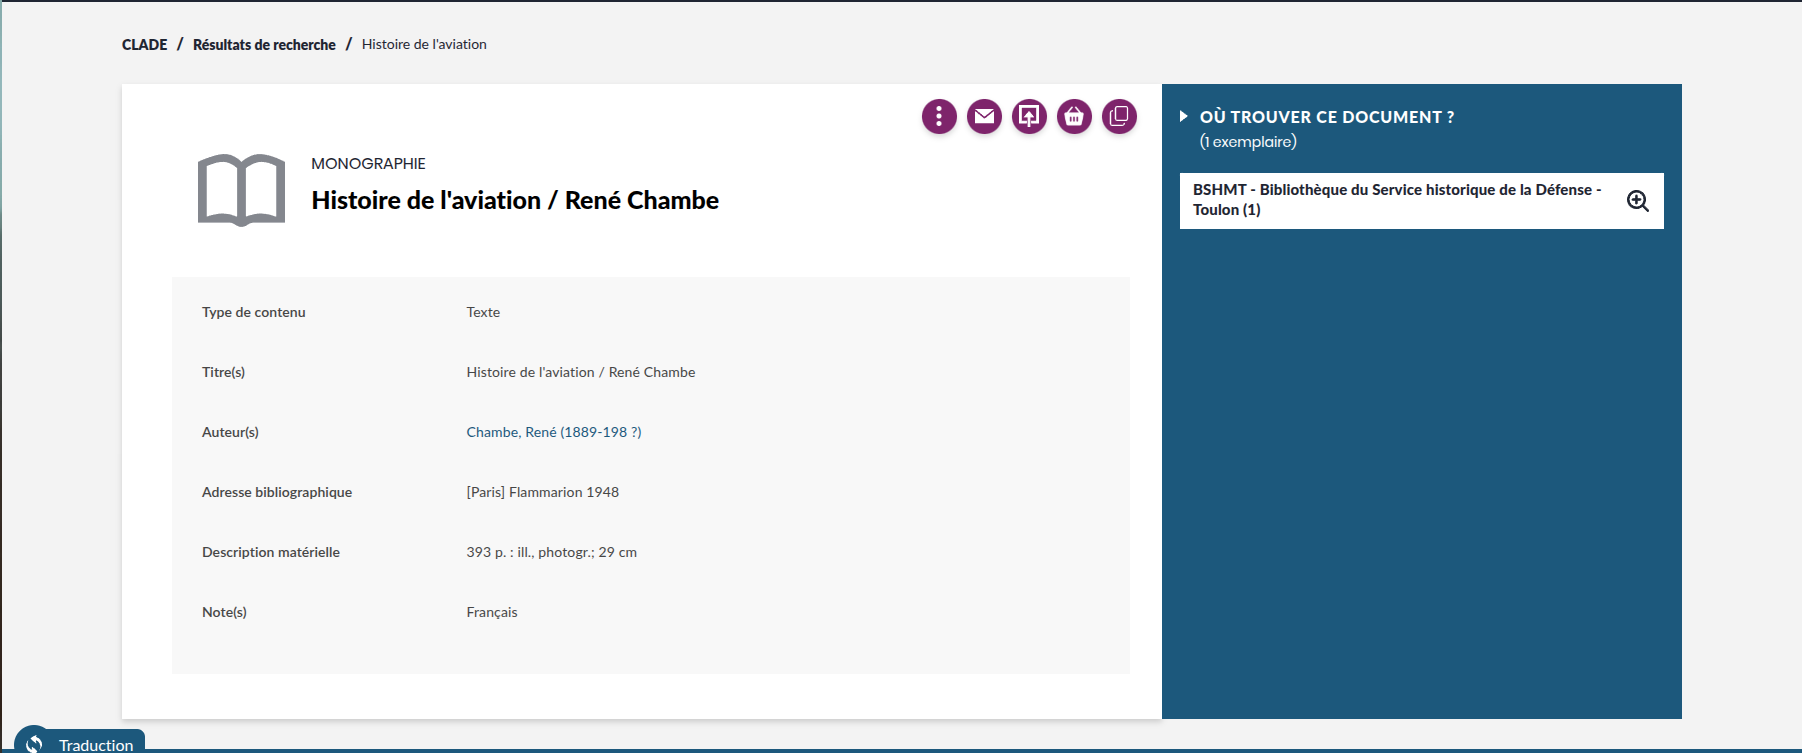
\includegraphics[width=\linewidth]{img/IMG_clade_histoireaviation_shdTL}
		\caption{Service Historique de la Défense}
		\label{img:cladehistoireaviationshdtl}
	\end{subfigure}
	\begin{subfigure}{0.7\textwidth}
		\centering
		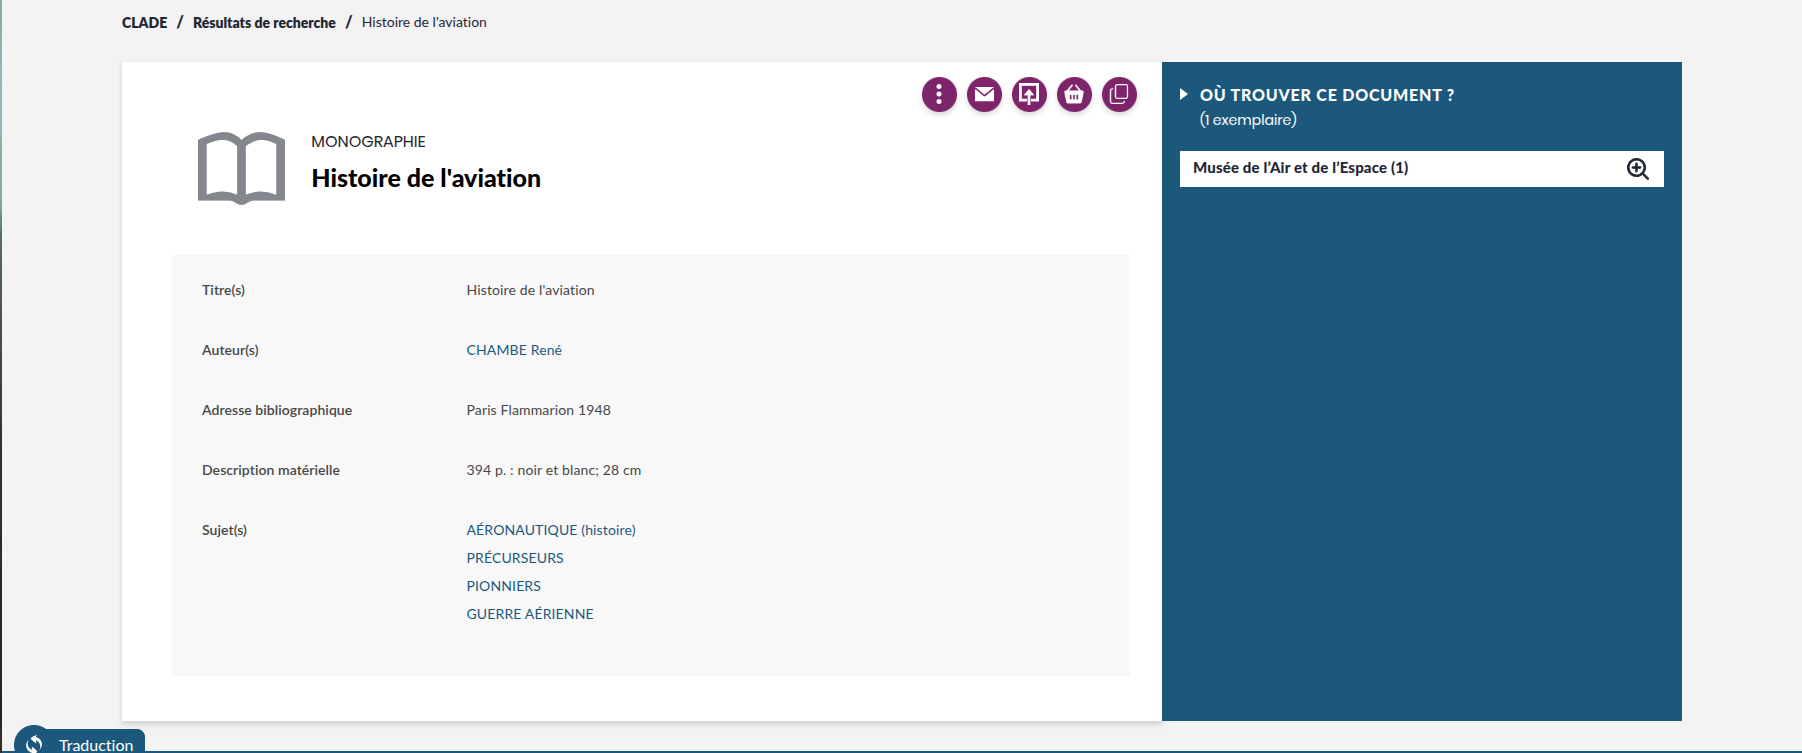
\includegraphics[width=\linewidth]{img/IMG_clade_histoireaviation_mae}
		\caption{\mae}
		\label{img:cladehistoireaviationsmae}
	\end{subfigure}
	\hfill
	\begin{subfigure}{0.7\textwidth}
		\centering
		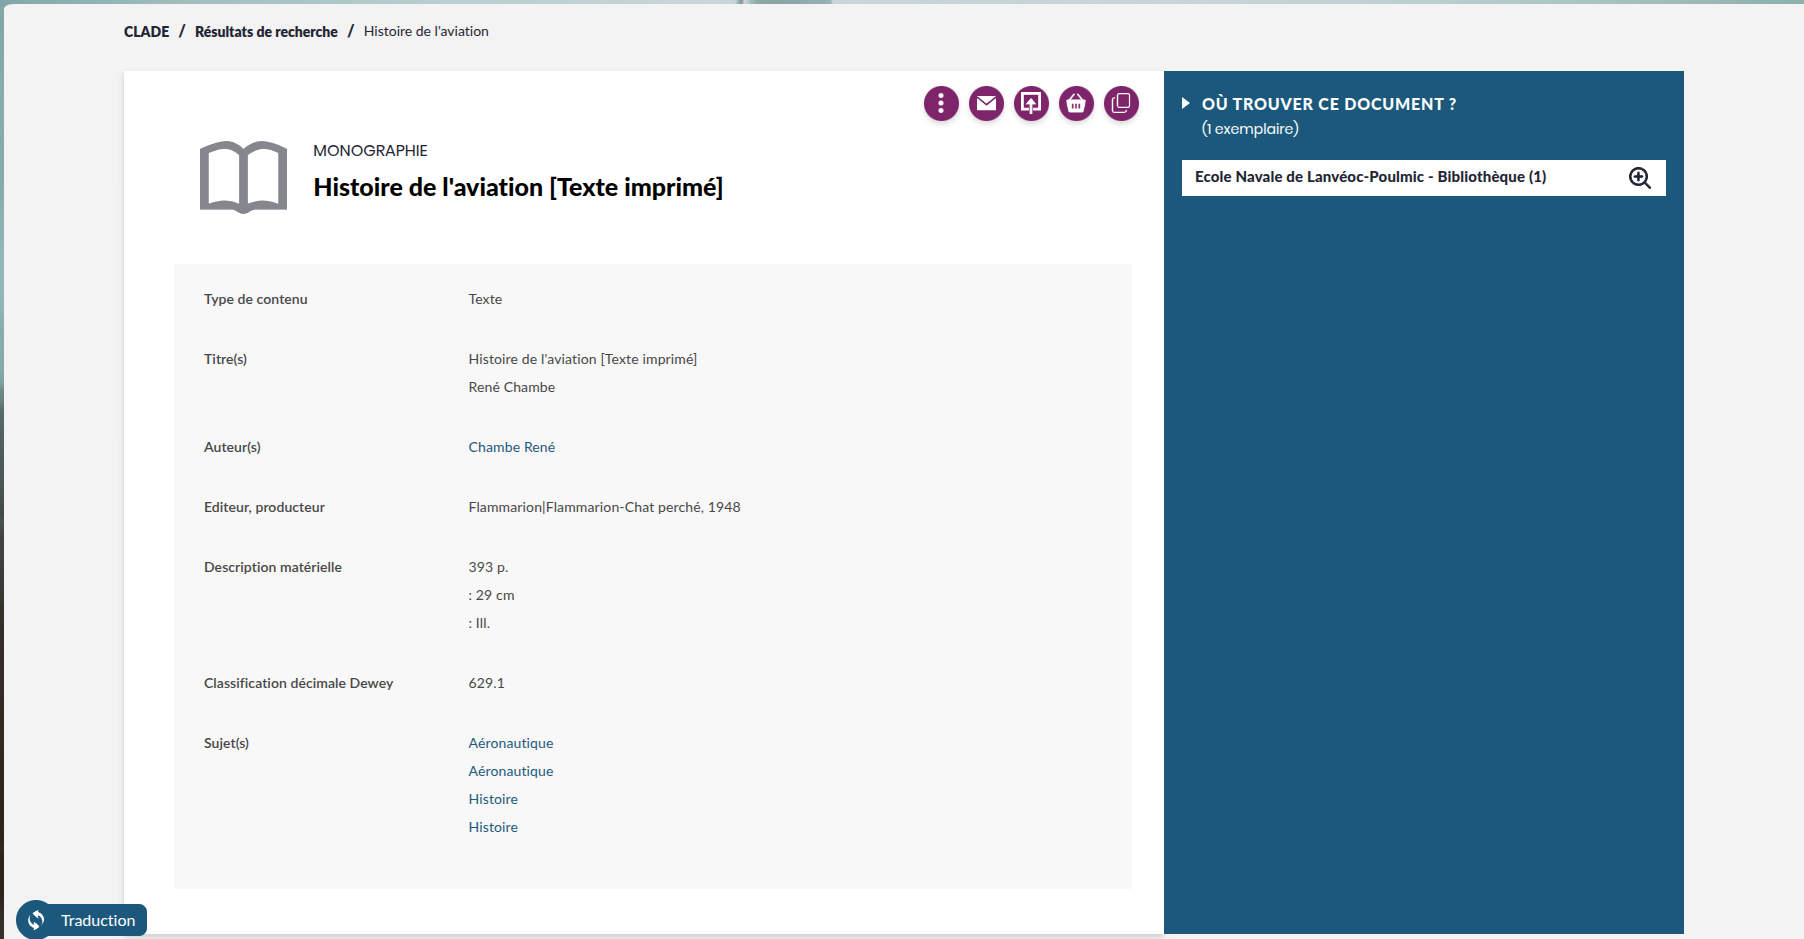
\includegraphics[width=\linewidth]{img/IMG_clade_histoireaviation_navale}
		\caption{École navale}
		\label{img:cladehistoireaviationnavale}
	\end{subfigure}
	\caption[Différences de catalogage entre les \bibmusee sur \ac{clade}]{Malgré la volonté de mise en commun sur \ac{clade}, la même édition d'un même ouvrage peut être cataloguée de plusieurs manières différentes et apparaître comme des ouvrages distincts : ici, l'\textit{Histoire de l'aviation} de René Chambe chez Flammarion (1948).} On remarquera les différences entre les captures \ref{img:cladehistoireaviationnavale} et \ref{img:cladehistoireaviationsmae} concernant les \enquote{sujets} indexés : ce sont eux qui constituent l'essentiel des \gls{thesaurus} du \mae.
	\label{fig:clade_histoaviation}
\end{figure}

Ce cas illustre parfaitement les tensions inhérentes aux vocabulaires contrôlés en contexte institutionnel contraint : l'harmonisation impose des choix qui peuvent entrer en conflit avec les besoins documentaires spécifiques, et pose la question de trouver comment accorder les richesses des connaissances de chaque institution concernée avec la nécessité d'avoir un minimum d'uniformité lorsqu'il s'agit de coopérer à grande échelle. Cette expérience pose des questions que nous développerons dans les parties suivantes : quels critères peuvent guider la conception de vocabulaires contrôlés qui articulent contraintes institutionnelles et exigences scientifiques ? Comment évaluer les compromis entre interopérabilité et précision sémantique, et fidélité à l'identité et à la valeur scientifique des collections ?

\bigskip
\bigskip
\bigskip

\lettrine{L}{e} \maelong, musée de France doté d’un statut prestigieux et d’un patrimoine exceptionnel, évolue ainsi dans un cadre institutionnel et administratif fortement marqué par sa dépendance au ministère des Armées. Cette situation conditionne ses choix stratégiques, ses ressources, mais aussi son identité culturelle : le tout reflétant à la fois les contraintes spécifiques d’un établissement public militaire et les enjeux généraux liés à la conservation et à la valorisation de la mémoire aéronautique civile et militaire française. 

\bigskip
\bigskip
\bigskip
	
	%%%%%%%%%%%%%%%%%%%%%%%%%% CONCLUSION %%%%%%%%%%%%%%%%%%%%%%%%%%
	
	\lettrine{I}{ci}, je pourrai mettre la conclusion de cette partie
	
	%%%%%%%%%%%%%%%%%%%%%%%%%%% PARTIE II %%%%%%%%%%%%%%%%%%%%%%%%%%%%
	%%%%%%%%%%%%%%%%%%%%%%%%%%%%%%%%%%%%%%%%%%%%%%%%%%%%%%%%%%%%%%%%%%
	
	\part{La prolifération de l'information en institution culturelle, un sujet facilement mis de côté}
	
	%%%%%%%%%%%%%%%%%%%%%%%%%% INTRODUCTION %%%%%%%%%%%%%%%%%%%%%%%%%%
	
	Ici, je pourrai mettre une introduction de ma première partie
	
	%%%%%%%%%%%%%%%%%%%%%%%%%%%%% TEXTE %%%%%%%%%%%%%%%%%%%%%%%%%%%%%%
	
	\chapter[Les vocabulaires contrôlés au \ac{mae}]{\label{II-A} Multiplication et fragmentation des vocabulaires au \ac{mae}}

\begin{quote}
	\og Il se prépara un grand vocabulaire, et attendit toute la vie une idée\footcite{barney_pensees_1920}.\fg
\end{quote}

\lettrine{G}érer un musée, une bibliothèque ou un projet de recherche, c’est toujours se confronter au savoir : à sa dispersion, à sa multiplicité, à son épaisseur. Et cette confrontation impose un choix – celui des termes, de leur agencement, de la structure qui en découle. Ces choix ne sont jamais neutres : ils fondent la manière dont l’institution comprend ses collections, les articule, les rend lisibles. Le \ac{mae}, comme d’autres musées, a ressenti très tôt le besoin de maîtriser son langage descriptif, en construisant des vocabulaires contrôlés, d’abord localement, puis de manière plus ambitieuse, mais sans réelle coordination d’ensemble.

\section{\label{II-A-1}Une construction séparée : 25 ans d'évolution en silo}

Ici, du texte

\section{\label{II-A-2}Des conséquences importantes : quand la prolifération devient paralysie documentaire}

L’exercice de diagnostic mené sur les thésaurus du \mae révèle que plus l’institution enrichit ses descriptions, plus elle complexifie l’accès à ses propres collections. Cette prolifération de vocabulaires entraîne des complications, incitant les chargés de collections et documentalistes à reconsidérer leurs méthodes actuelles. L’observation de terrain révèle deux manifestations principales de cette dégradation : l’invisibilisation progressive des collections et la saturation dans l’organisation des équipes, ces deux facteurs contribuant à rendre plus difficile encore toute rationalisation de l’accumulation d’information au musée.

\subsection{L’invisibilisation documentaire : effet direct de la fragmentation des vocabulaires}

L’un des défis relevé à plusieurs reprises dans les échanges avec les agents du \mae est la difficulté croissante à retrouver certains documents ou objets, malgré l’enrichissement constant des vocabulaires. Cette situation ne tient pas seulement à la prolifération des termes, mais à leur organisation disjointe : la coexistence de thésaurus parallèles et non coordonnés enferme les informations dans des silos que rien ne relie. Cette fragmentation est notamment étudiée par Richard Gartner et Raphaëlle Mouren dans un article sur la méthodologie mise en place pour éviter ces écueils à la Warburg Institute Library. Bien que le contexte technologique ne soit pas exactement le même, cette analyse s’applique également au \mae : les différences de vocabulaires y sont surtout liées aux différences de conception des métadonnées en général entre les métiers des archives, des musées et des bibliothèques. Même si le musée n’utilise pas les mêmes standards, la citation reste pertinente :  

\begin{quote}
	\og Il existe très peu d’interopérabilité entre ces trois approches, et par conséquent entre leurs communautés respectives, en raison de leurs architectures sous-jacentes distinctes, elles-mêmes issues de conceptions très différentes des métadonnées qui se sont développées depuis des siècles au sein de chaque secteur. En l’absence de cette interopérabilité, il devient difficile de favoriser la découvrabilité entre différents secteurs ou intercommunautaire, et donc de permettre aux utilisateurs des archives ou des musées d’accéder aux précieuses ressources patrimoniales conservées, par exemple, dans le secteur des bibliothèques\footcite{gartnerArchivesMuseumsLibraries2019}.\fg
\end{quote}

Au \mae, cette situation se concrétise par le fait qu’une information (par exemple, un modèle d’avion rattaché à son constructeur) se retrouvera dans le thésaurus des aéronefs de l’\gls{emediatheque} et non dans la table des constructeurs de \gls{micromusee}, et le chercheur voulant accéder à la totalité des connaissances détenues par l’institution sur le sujet doit penser aux différents moyens d’accès disponibles dans chaque cas.

La manière d’organiser l’information est tout aussi importante que son contenu : au \mae, où de nombreuses imprécisions ou erreurs sont restées sans correction, il devient difficile d’accéder à certains documents en utilisant des mots-clés qui seraient pourtant intuitifs. Par exemple, une recherche géographique dans l’\gls{emediatheque} : une photographie indexée sous un nom de ville devrait pouvoir apparaître lors d’une recherche par région. Or, dans la branche « lieux » des mots-clés de l’\gls{emediatheque}, le terme générique direct est un pays et non une région ; il en résulte qu’une photographie indexée sous « Pont-l’Évêque » rattachée directement à « France » ne sera pas retrouvée par un chercheur interrogeant le fonds sous « Normandie » ou « Calvados ». De même, de nombreux objets techniques, catalogués avec des dénominations précises propres au monde de l’aéronautique, échappent aux requêtes du grand public, qui n’en connaît pas le vocabulaire.

Cette problématique rejoint une exigence ancienne du métier de documentaliste, brillamment formulée par Magdeleine Moureau dès 1968 :

\begin{quote}
	\og En outre chaque document doit pouvoir satisfaire aux deux objectifs documentaires : diffusion systématique et recherche sur question, et pouvoir restituer le même document lors d’une question générique ou lors d’une question spécifique. Cette possibilité de répondre à plusieurs niveaux pourra s’obtenir de deux façons : soit par l’indexateur humain qui rajoutera pour chaque document particulier le thème général dont il procède, soit par la machine qui associera automatiquement certaines notions génériques à certaines notions spécifiques, par exemple Europe à France ou aromatique à benzène\footcite{moureauProblemesPosesPar1968}.\fg
\end{quote}

L’utilisation d’un thésaurus est l’outil choisi dans les années 1990 par le \mae pour répondre à ces objectifs. Son passage au second plan pendant les dernières décennies impacte donc directement ces deux « objectifs documentaires » et muséaux.

Cette invisibilisation n’est pas une fatalité : elle invite à repenser la coordination des vocabulaires et à développer des outils de recherche capables de traverser ces silos, en mobilisant les méthodes de normalisation et d’interopérabilité proposées par les dernières normes ISO\footcite{chichereauNormesConceptionGestion2007}.

\subsection{La saturation des métiers : quand gérer devient ingérable}

Au quotidien, on observe que l’adéquation des outils de gestion documentaire reste un enjeu central pour les équipes du musée. Par exemple, la version 6 de \gls{micromusee}, logiciel développé dans les années 1990 et resté en usage jusqu’en 2025, a été souvent décrite comme « antique » par ses utilisateurs : ce cas illustre bien les difficultés d’adaptation et de gestion auxquelles ont été confrontés les agents face aux limites ou à la présentation de certains outils. Ce logiciel présentait toutes les fonctionnalités nécessaires pour la gestion des collections : gestion des notices, modification par lot, gestion de thésaurus... mais il était devenu difficile à lancer sur des systèmes d’exploitation actuels, très peu ergonomique, et surtout n’offrait aucune possibilité d’interopérabilité avec d’autres logiciels. La migration vers \gls{archange} a ainsi nécessité l’engagement d’un renfort informatique pour traiter les nombreux fichiers texte en ASCII exportés de la base et les transposer dans des fichiers csv plus lisibles et transmissibles au prestataire de migration.

Comme le souligne Hélène Vassal dans l'ouvrage \citetitle{merleau-pontyDocumenterCollectionsMusees2016}, « l’accès aux œuvres passe aussi par l’accès à leur connaissance », et cet accès passe aujourd’hui par des outils informatiques qui \enquote{[rendent] l’utilisation des bases de données et de leurs applications indissociables des pratiques quotidiennes des professionnels de la documentation et de la régie\footcite{merleau-pontyDocumenterCollectionsMusees2016}.} Le volume des données concernées, souvent en milliers de mots, n’est pas toujours traitable pièce à pièce par l’humain.

Cependant, comme le rappelle Maryse Rizza dans \citetitle{rizzaDocumentAuCoeur2014}, le numérique n’est pas un but en soi et il est \enquote{au service du musée et de ses missions\footcite{ricardRGPDArchives2018a}}. Cette évolution transforme néanmoins profondément l’exercice des métiers muséaux en imposant \enquote{un élargissement des compétences pour les professionnels de musée qui assurent le traitement documentaire des documents numériques\footcite{rizzaDocumentAuCoeur2014}.}. Cette tension entre l’expertise approfondie que requiert la gestion de vocabulaires spécialisés, et la dispersion des compétences qu’impose la multiplication des systèmes, se retrouve aujourd’hui au \mae. Les agents du \ac{drd} doivent maîtriser simultanément \gls{koha} et l’\gls{emediatheque}, et se familiariser avec le nouvel outil de gestion des collections muséales \gls{archange}. La gestion de thésaurus — et surtout le chantier de nettoyage, mise aux normes, et migration vers un logiciel pour faciliter son exploitation — se surajoute aux missions des agents, en leur demandant d’acquérir de nouvelles compétences et de dégager du temps pour s’y consacrer. Il en est de même pour la gestionnaire de base de données côté musée, pour qui ce travail s’ajoute à ses missions d’origine.

L’organisation de l’information au musée, que ce soit au travers de la gestion d’un thésaurus ou autre, représente des défis métiers majeurs :
\begin{itemize}
	\item Cette gestion revient à manipuler des masses considérables de données, ce qui demande un temps de travail que n’ont pas nécessairement les agents à qui reviendrait plus naturellement ce rôle,
	\item elle dépend très étroitement de la qualité des outils mis à leur disposition,
	\item et demande de se former continuellement à des pratiques toujours en évolution.
\end{itemize}

\bigskip
\bigskip
\bigskip

Cette rapide analyse des dysfonctionnements rencontrés au \mae quant à la gestion de l'information révèle que sa prolifération pose un véritable problème de gouvernance intellectuelle. Ce n’est pas tant la quantité de données qui paralyse l’institution, même si elle joue sur la charge de travail que représente toute gestion de l'information, que l’absence de coordination entre les systèmes de description. Face à cette fragmentation, le thésaurus unique s’impose comme un instrument privilégié d’organisation de l’information, mais sa mise en œuvre suppose de dépasser les clivages métiers et d’inventer de nouvelles formes de collaboration intellectuelle.


\bigskip
\bigskip
\bigskip

Et ici, une conclusion.
	\chapter[PDV métier]{\label{II-B}Des rôles et une prise de conscience différenciée selon les métiers }

\lettrine{L}a fragmentation des vocabulaires contrôlés au sein du \maelong ne s'explique pas seulement par la diversité des outils ou des collections. Elle traduit une histoire institutionnelle où chaque métier — documentaliste, gestionnaire de base de données, chargé de collections — a développé sa propre sensibilité à la question du vocabulaire. Cette pluralité, loin d'être accidentelle, témoigne d'une répartition différenciée des rôles, des responsabilités et des rapports à l'information, qui conditionnent aujourd'hui la possibilité d'une gouvernance documentaire commune.

\section{\label{II-B-1}Une montée du besoin de réflexion sur le vocabulaire du musée différenciée selon les métiers }


Prise de conscience d'abord par les documentalistes, qui ont déjà des habitudes de construction de thésaurus et pour qui la question de l'interopérabilité se pose plus au quotidien (projets d'intégration au sudoc, SIGB commun, recherche de visibilité pour attirer les lecteurs/chercheurs, volonté de mettre en avant un fonds particulier) 

Gestionnaire de base de données : de par son métier, prise de conscience directe de la nécessité d'harmoniser le contenu des notices, d'avoir un référentiel pour indexer. Chargée d'aller elle-même modifier dans la BDD quand changement de terminologie 

Un sujet qui a été mis sur le tapis grâce aux migrations (changement de SIGB pour la bibliothèque, changement de logiciel de gestion des collections pour le musée) 

Chargés de collection, une relation ambigue : Une sensibilité qui dépend principalement de l’usage quotidien qui en est fait et des besoins ponctuels. 

Une sensibilité qui dépend aussi d’une conception de son métier : différents choix qui sont faits pour le thésaurus des domaines en particulier. 
\section{\label{II-B-2}Des différences d’appréhension qui traduisent un rapport très différent à l’information}

\subsection*{Problématisation générale}

La fragmentation des pratiques documentaires au sein des institutions patrimoniales — musées, bibliothèques, archives — est un objet de réflexion récurrent dans la littérature contemporaine sur la gouvernance de l'information. Elle ne relève pas d’un simple défaut de coordination, mais traduit des rapports fondamentalement divergents à la nature de l’information, à sa matérialité, à sa finalité et à ses usages. Cette diversité des appréhensions, loin d’être accidentelle, est le produit d’histoires institutionnelles, de cultures professionnelles et de logiques métiers distinctes\footcite{bowkerArrangerChosesConsequences2023,gartnerArchivesMuseumsLibraries2019,rizzaDocumentAuCoeur2014}.

\subsection*{1. Pluralité des priorités dans la description des œuvres}

Dans la littérature sur les vocabulaires contrôlés et la gouvernance documentaire\footcite{hudonISO25964Pour2012a,nouvelOutilsDindexationBibliothecaires2022,chichereauNormesConceptionGestion2007}, il est souvent rappelé que la description des œuvres ne répond pas à une logique unique :
\begin{itemize}
	\item Les musées privilégient la matérialité, l’histoire singulière de l’objet, son contexte d’usage et sa dimension patrimoniale. Le vocabulaire est alors pensé comme un outil au service de la spécificité et de l’exhaustivité.
	\item Les bibliothèques mettent l’accent sur la structuration sémantique, la traçabilité des concepts, la cohérence du langage documentaire. La finalité est l’accès, la recherche, la circulation de l’information.
	\item Les archives accordent une importance primordiale à la chaîne de production, à la preuve, à la traçabilité du document, et à la continuité institutionnelle.
\end{itemize}
Cette diversité engendre des priorités concurrentes, qui se manifestent dans la conception même des thésaurus et des systèmes d’indexation. Comme le rappelle Maryse Rizza\footcite{rizzaDocumentAuCoeur2014}, le document prend sens différemment selon qu’il est considéré comme œuvre, publication ou preuve administrative.

\subsection*{2. Enjeux d’interopérabilité et logiques métiers}

L’interopérabilité, souvent invoquée comme horizon commun des systèmes d’information patrimoniaux\footcite{hudonISO25964Pour2012a,bermesVersNouveauxCatalogues2016}, apparaît en réalité comme un besoin inégalement partagé :
\begin{itemize}
	\item Pour les documentalistes, elle est vitale : elle garantit la visibilité du fonds, la circulation des savoirs, la légitimité scientifique de l’institution.
	\item Pour les gestionnaires techniques, elle est une contrainte opérationnelle, imposée par les migrations logicielles ou l’intégration à des réseaux ministériels.
	\item Pour les chargés de collections, l’interopérabilité peut être perçue comme une menace pour la singularité des pratiques, ou comme un enjeu secondaire, mobilisé surtout lors d’expositions ou de projets transversaux.
\end{itemize}
L’exemple du programme C-ADER illustre cette tension : le thésaurus développé pour la recherche sur les dégradations des matériaux répond à des besoins spécifiques, sans exigence d’intégration documentaire avec le musée, même si ses résultats pourraient enrichir le vocabulaire institutionnel.

\subsection*{3. La persistance des silos institutionnels : musées, bibliothèques, archives}

La littérature sur la coopération interinstitutionnelle\footcite{gartnerArchivesMuseumsLibraries2019,rossini-paquetBibliothequesMuseesQuellesa,yarrowBibliothequesPubliquesArchives2008a} souligne que, malgré leur proximité intellectuelle et leur mission commune de transmission du patrimoine, musées, bibliothèques et archives demeurent séparés par des logiques professionnelles et des architectures techniques distinctes.
\begin{itemize}
	\item Cette séparation est à la fois physique (locaux séparés), intellectuelle (référentiels, normes et standards propres) et fonctionnelle (missions spécifiques, publics différents).
	\item Les tentatives d’unification documentaire se heurtent à la résistance des métiers, à la diversité des systèmes et à la difficulté de construire des vocabulaires communs.
\end{itemize}
Ce constat est d’autant plus frappant que de nombreuses institutions, comme le \mae, rassemblent sous un même toit musée, bibliothèque et archives, mais peinent à articuler une mémoire intellectuelle unifiée. Gartner \& Mouren\footcite{gartnerArchivesMuseumsLibraries2019} parlent de « silos de métadonnées » et de la difficulté à « favoriser la découvrabilité intercommunautaire » des ressources patrimoniales.

\subsection*{4. État de la recherche et pistes théoriques}

La littérature récente propose plusieurs pistes pour penser cette fragmentation :
\begin{itemize}
	\item Bowker \& Star\footcite{bowkerArrangerChosesConsequences2023} invitent à « explorer les conséquences de la classification », soulignant que toute structuration documentaire est le produit de choix politiques et organisationnels, qui laissent des traces dans la mémoire institutionnelle.
	\item Bermès\footcite{bermesVersNouveauxCatalogues2016} et Hudon\footcite{hudonISO25964Pour2012a} insistent sur la nécessité de concevoir des classifications flexibles, capables d’intégrer la diversité des usages et la pluralité des acteurs.
	\item Nouvel\footcite{nouvelOutilsDindexationBibliothecaires2022} et Chichereau\footcite{chichereauNormesConceptionGestion2007} rappellent que l’interopérabilité ne peut être pensée sans une réflexion sur les rapports de pouvoir et la reconnaissance des expertises métiers.
\end{itemize}

Enfin, la question de l’unité intellectuelle des institutions patrimoniales reste ouverte : les solutions techniques (modélisation, alignement de vocabulaire, normes SKOS/ISO) ne suffisent pas à abolir les différences d’appréhension — elles doivent s’accompagner d’une réflexion institutionnelle et d’une politique documentaire ambitieuse.

\subsection*{Transition}

Il apparaît ainsi que la fragmentation des pratiques métiers dans la gestion de l’information patrimoniale ne relève pas seulement d’un problème technique, mais d’une pluralité de rapports à l’information, à la valeur patrimoniale, et à la mission de transmission. Les solutions envisagées dans la littérature appellent à une prise de conscience de cette diversité, préalable à toute tentative d’unification documentaire.

\bigskip
\bigskip
\bigskip

\lettrine{L}{a} diversité des métiers et des rapports à l'information au \mae engendre une fragmentation des vocabulaires et des pratiques documentaires, qui complique la mise en œuvre d'une gouvernance commune. Comprendre ces clivages professionnels, articuler les priorités divergentes et mobiliser les apports de la littérature académique constitue un préalable incontournable à toute politique d'unification documentaire. La réflexion sur l'interopérabilité et la mémoire organisationnelle, loin d'être un simple enjeu technique, est au cœur de la transmission patrimoniale et de la valorisation scientifique des collections du musée. 
	\chapter[Les archives numériques]{\label{II-C}Les archives numériques : une autre manifestation des difficultés de gestion de l’information en musée }

\begin{quote}
	\enquote{\textbf{ARCHIVES INFORMATIQUES} \textit{en : electronic records}
		Documents produits ou reçus par un organisme dans l'exercice de
		ses activités et conservés sous forme d'enregistrements
		électroniques sur des supports tels que les bandes magnétiques,
		les disques magnétiques, les disques optiques etc., et qui ne
		peuvent être lus que par l’intermédiaire d’une machine\footcite{directiondesarchivesdefranceDictionnaireTerminologieArchivistique2002}.}
\end{quote}

\lettrine{D}{ans} le musée, la question des archives numériques est à la croisée des chemins : entre mémoire documentaire et gestion administrative, elle met en lumière l’ambiguïté qui sépare – ou confond – archives et documentation. Cette frontière est souvent difficile à définir dans le milieu des musées et, loin d’être purement technique ou juridique, elle recouvre des enjeux de gouvernance, de responsabilité et de pérennité du savoir dans un contexte où la masse des données numériques croît plus vite que ne se structurent les pratiques. L’expérience du \mae, qui se révèle dans son organigramme comme dans sa pratique quotidienne – où l’unique archiviste ne peut déjà embrasser la diversité des fonds papier – illustre les dilemmes contemporains de l’archivage en musée. Comment garantir la pérennité et la communicabilité des archives publiques numériques d'un musée lorsque la distinction entre archive et document est floue, quand l’outil et les référents professionnels manquent, et quand la réflexion collective reste à construire de zéro ? 

Dans une première partie, nous tâcherons d'examiner les ressorts de cette frontière incertaine entre archives et documentation qui existe en contexte muséal, en interrogeant les pratiques, les outils et les propositions institutionnelles pour tenter d'y pallier. Puis, dans une seconde partie, nous porterons l’analyse sur la figure de l’archiviste en musée, dont la légitimité s’avère difficile à établir : nous mettrons en lumière les enjeux techniques, juridiques et professionnels qui entravent la mise en place d’une véritable politique d’archivage raisonné, et les difficultés spécifiques que soulève la gestion quotidienne des archives numériques par des agents souvent peu formés et insuffisamment sensibilisés à la gouvernance documentaire.

%\lettrine{D}{ans} le paysage contemporain des institutions patrimoniales, la question des archives numériques se dresse avec une acuité nouvelle, révélant en creux les tensions qui traversent le quotidien des musées techniques. Au Musée de l’Air et de l’Espace, où la mémoire documentaire s’entrelace étroitement avec la gestion courante, la technicité des outils informatiques se heurte à la faiblesse des moyens humains, et la pratique quotidienne à la rigueur réglementaire. La frontière — déjà ténue — entre archives et documentation s’y révèle d’autant plus poreuse que l’institution ne dispose que depuis peu d’une archiviste dédiée. Il importe alors, pour comprendre les logiques qui entravent la mise en œuvre d’une gouvernance archivistique digne de ce nom, d’interroger la dialectique entre impératifs institutionnels, contraintes techniques, et réalités humaines, sous le prisme de la littérature professionnelle et du vécu des agents.
\section{La frontière floue entre archives et documentation : une problématique propre aux musées techniques}

\subsection{Définir l’archive numérique en contexte muséal : enjeux et ambiguïtés}

%Les musées en France, institutions dédiées à la conservation et à la diffusion du patrimoine, sont intimement liés à la question des archives : eux-même producteurs d'archives, ils peuvent être également exceptionnellement appelés à en être les dépositaires lorsqu'elles sont indissociables d'une oeuvre. Malgré la prégnance des problématiques liées à la gestion des archives dans les musées dans le paysage français, la littérature scientifique et professionnelle sur ce sujet semble peu prolifique : l'article de référence que nous retiendrons pour ce développement est celui de Véronique Sassetti-Aguilera, \citetitle{sassetti-aguileraArchivesMuseesDiversites2020a}. L'autrice identifie trois problématiques principales dans les musées actuellement : \enquote{La première difficulté réside dans le statut même de l'établissement (public ou privé) qui caractérise le plus souvent la nature des fonds d'archives et des collections [...] La deuxième, nettement plus complexe, relève de l'identification des archives par le personnel des musées comme trésors nationaux, imprescriptibles et inaliénables [...] La troisième enfin, et non la moindre, demeure dans l'enrichissement continuel de la documentation scientifique des collections de musées, situation ne permettant jamais [...] de procédures d'archivage classiques par bordereaux de versement.}. Ces problématiques se retrouvent au \mae. Celui-ci est en effet une institution publique, l'ensemble de ses archives sont donc est celle de la frontière : où finit la documentation, où commence l'archive ? Cette interrogation, classique en archivistique, se complique singulièrement dans l'environnement numérique muséal, où la nature hybride des fonds — documents de gestion, dossiers d'œuvre, photographies, fichiers bureautiques, bases de données — brouille irrémédiablement les distinctions traditionnelles.

\begin{itemize}
	\item \textbf{Problématique} : Qu’est-ce qu’une archive numérique en musée ? En quoi la nature hybride des fonds (documents de gestion, dossiers d’œuvre, photographies, fichiers bureautiques, bases de données) brouille-t-elle la distinction entre documentation courante et archives ?
	\item \textbf{Pistes d’analyse} : 
	\begin{itemize}
		\item Définitions normatives (\textit{archive courante, intermédiaire, définitive}, cf. Code du patrimoine, FICHE\_Information\_Archivistique.md).
		\item Spécificité muséale : la documentation devient archive dès lors qu’elle sert à la mémoire du musée ou à la justification de ses droits.
		\item Les dossiers d’œuvre : archives ou documentation ? \footcite{barbelinDossierDoeuvreDossier2016a}
		\item Données numériques et patrimonialisation de l’information technique \footcite{bechardArchivesElectroniques2020a}
	\end{itemize}
	\item \textbf{Exemples concrets} : Dossiers d’œuvre (archives-administration, rapports, photographies, courriels, cf. FICHE\_Information\_Archivistique.md), photographies de la médiathèque, rapports d’activité.
	\item \textbf{Citation} : \og Les dossiers d’œuvre sont des archives publiques : ils sont librement communicables à tout citoyen. \fg \footcite{barbelinDossierDoeuvreDossier2016a}
\end{itemize}

\subsection{Panorama des pratiques de gestion des archives numériques au MAE}

\begin{itemize}
	\item \textbf{Problématique} : Où et comment sont conservés les fichiers numériques ? Quelles logiques d’organisation ? Quelles difficultés concrètes ?
	\item \textbf{Pistes d’analyse} :
	\begin{itemize}
		\item Cartographie des espaces de stockage : Serveur S (archives courantes, arborescence par service, gestion Windows Explorer), SharePoint, OneDrive.
		\item Hétérogénéité des usages et compétences, conséquences sur la pérennité.
		\item Problèmes récurrents : arborescence trop ou trop peu granulaire (cf. FICHE\_RAPPORT\_ServeurS.md), doublons, conventions de nommage non pérennes (nuage de mots, FICHE\_Bonnes\_Pratiques.md), noms au nom des agents (cf. FICHE\_Photos.md), absence de plan de classement partagé.
		\item Conséquences : invisibilisation, perte de repères, saturation.
	\end{itemize}
	\item \textbf{Exemples concrets} : Ratio fichiers/dossiers, arborescence profonde (16 niveaux, cf. FICHE\_RAPPORT\_ServeurS.md), nommage des photos et vidéos (cf. FICHE\_Photos.md), dossiers « vrac » (FICHE\_Bonnes\_Pratiques.md).
	\item \textbf{Citation} : \og Un bon classement = une information trouvable, fiable et partageable durablement. \fg (FICHE\_Bonnes\_Pratiques.md)
\end{itemize}

\subsection{Un personnel sous-dimensionné : la difficile reconnaissance de la fonction archivistique}

\begin{itemize}
	\item \textbf{Problématique} : Pourquoi la fonction archivistique reste-t-elle marginale dans les musées techniques ? Quelles conséquences sur la gestion des archives numériques ?
	\item \textbf{Pistes d’analyse} :
	\begin{itemize}
		\item Une seule archiviste au MAE depuis 2024, principalement dédiée aux archives privées papier.
		\item Rattachement à la documentation : dilution des missions, surcharge, arbitrages constants.
		\item Absence de politique de formation et de sensibilisation des personnels non archivistes (cf. FICHE\_Information\_Archivistique.md).
		\item Difficulté à établir plan de classement, tableau de gestion, chaîne archivistique.
	\end{itemize}
	\item \textbf{Exemples} : Missions d’archives ponctuelles, gestion dossiers d’œuvres, documentation.
	\item \textbf{Citation} : \og La distinction entre archives et documentation est remarquablement posée, [...] la gestion purement administrative des dossiers d’acquisition permet une uniformisation des pratiques. Peut-on à partir de cet exemple réfléchir à l’élaboration de procédures spécifiques en matière d’archives publiques de musées en France ? \fg \footcite{sassetti-aguileraArchivesMuseesDiversites2020a}
\end{itemize}


\section{\label{II-C-2}Vers une gouvernance des archives numériques au \mae : expérimentations, structuration et montée en compétences}


\begin{myquote}
	{Ne pas envisager l’archivage de documents numériques dès leur création, c’est prendre le risque de les perdre définitivement.}{ministeredelacultureArchivesElectroniquesDans2020}
\end{myquote}

\subsection{Quelques leviers}


Loin de se réduire à une succession d’obstacles, la situation des archives numériques au musées est aussi un terrain privilégié pour tenter une réconciliation des dynamiques muséales et archivistiques. Les recommandations nationales – garantie de l'intégrité du fichier et de ses métadonnées, distinction des états d’archives, traçabilité, bordereaux d’élimination – sont peu à peu reconnues, d'abord par le \ac{drd}, sensibilisé par ses missions aux enjeux de gestion de l'information, puis par les agents du \ac{dsc} qui y sont confrontés au quotidien.



Certes, la question du versement définitif demeure ouverte : aucun projet d'intégration immédiate à un \gls{sae} ne paraît envisageable, mais la problématique est reconnue, et il faut reconnaître que la priorité est donnée pour l'instant aux chantiers logiciels menés par le \minarm (\gls{koha}-\gls{clade} et \gls{archange}), reléguant la question de l’archivage à une temporalité indéfinie. La sensibilisation des agents se heurte à la dispersion des responsabilités et la fonction archivistique demeure fragile, mais des quelques avancées pour poser les bases de projets ultérieurs plus conséquents ont été proposées au \ac{dsc}, qui pourrait alors, après une première expérimentation, argumenter pour un chantier commun à l'ensemble du musée.


La première, et l'une des missions secondaires de ce stage, a consisté en la production de moyens de sensibilisation des agents du \ac{dsc} aux enjeux de gouvernance de leurs archives numériques : ceux-ci auront consisté principalement en 
\begin{itemize}
	\item la réalisation de formations de sensibilisation à l’adresse des agents,
	\item la rédaction d’une Foire aux Questions sur la gestion quotidienne et les grands principes d'archivistique[TODO : ajout annexe faq caviardée],
	\item la production de fiches de bonnes pratiques.
\end{itemize}

La seconde, liée à la précédente, est le recueillement des ressentis et des pratiques déjà en vigueur dans le service, afin de proposer des solutions réalistes et adaptées aux exigences métier : cette démarche a abouti à la proposition de normes de nommages de fichiers et de dossiers, et de structuration de l'arborescence générales au service et à la création d'un document partagé de mise en commun du vocabulaire et des abréviations utilisées.


Il s’agit ici d’insuffler une culture commune de la gestion documentaire : nommage, tri, organisation, bordereaux d’élimination sont pensés comme autant de jalons vers une maîtrise accrue du cycle de vie des fichiers. Face à l’impossibilité actuelle d’un archivage définitif, l'engagement d'un professionnel dédié au tri du serveur, à la validation des éliminations et à la mise en conformité des procédures est souhaitable ; dans l'attente d'une solution institutionnelle, une réflexion s’est engagée sur la création d’un dossier réservé à l'archivage des documents arrivés à leur fin d'utilité administrative.


Pour préparer le terrain d'une gestion robuste de ses archives, ces initiatives, portées par le \ac{dsc} illustrent la possibilité d’entamer une dynamique de modernisation fondée sur la formation, l’accompagnement et l’engagement des agents, même en l’absence de dispositifs techniques pleinement aboutis.

\bigskip
\bigskip
\bigskip

La crise de l’archivage numérique en musée ne se résume pas à une accumulation de défauts : elle révèle également la capacité de l’institution à inventer des solutions pour organiser sa gouvernance en conformité avec les recommandations en vigueur et former ses agents. Là encore, ce sont les métiers de la documentation, plus sensibilisés aux enjeux de la gouvernance de l'information en général qui sont à l'initiative de ces projets.

\bigskip
\bigskip
\bigskip

\lettrine{S}{ynthétiser} la crise de l’archivage numérique en musée, c’est reconnaître la fragmentation des espaces, la gouvernance éclatée, le sous-dimensionnement humain, et l’absence de solutions pérennes. Le cas muséal, singulier, se situe à la croisée des chemins : entre documentation et archives, le musée est sommé d’inventer une mémoire numérique qui soit fidèle à son histoire et adaptée à ses contraintes.

La nécessité d’une politique globale de gouvernance de l’information s’impose, pour que la mémoire numérique du MAE ne se dissolve pas dans le flux des fichiers et des tâches. Structuration, concertation, formation, sont les jalons à poser pour qu’à l’avenir, la mémoire du musée ne devienne pas l’otage de l’urgence, mais le reflet d’une institution soucieuse de son passé autant que de son devenir.
	
	%%%%%%%%%%%%%%%%%%%%%%%%%%% CONCLUSION %%%%%%%%%%%%%%%%%%%%%%%%%%%
	
	Ici, je pourrai mettre la conclusion  de cette partie.
	
	%%%%%%%%%%%%%%%%%%%%%%%%%%% PARTIE III %%%%%%%%%%%%%%%%%%%%%%%%%%%
	%%%%%%%%%%%%%%%%%%%%%%%%%%%%%%%%%%%%%%%%%%%%%%%%%%%%%%%%%%%%%%%%%%
	
	\part{Gérer la prolifération. Outils et méthodes}
	
	
	%%%%%%%%%%%%%%%%%%%%%%%%%% INTRODUCTION %%%%%%%%%%%%%%%%%%%%%%%%%%
	
	Ici, je pourrai mettre une introduction de ma première partie
	
	%%%%%%%%%%%%%%%%%%%%%%%%%%%%% TEXTE %%%%%%%%%%%%%%%%%%%%%%%%%%%%%%
	
	\chapter[Gérer la prolifération]{\label{III-A} Gérer la prolifération : outils et méthodes}



\lettrine{I}ntro

\section[La modélisation]{\label{III-A-1}La représentation conceptuelle : modéliser pour maîtriser la complexité}

\subsection{Les enjeux de la modélisation conceptuelle}

\paragraph*{Visualiser pour comprendre : le dévoilement des structures cachées}
Comme démontré plus haut dans la rapide présentation des vocabulaires utilisés au \mae, la masse de données à traiter est considérable\footnote{Voir le tableau \refinterne{tab:thesaurus_synthese}}. Ces données se présentent toutes sous la forme de tableurs excel exportés des différents logiciels de gestion du vocabulaire, et analyser leur structure et en déduire une méthodologie à suivre pour les optimiser est un réel défi pour le cerveau humain. Avant tout projet d'unification, visualiser les données pour pouvoir mieux les appréhender s’impose donc comme un nécessité : en effet, en les mettant à plat les et en permettant à l'utilisateur de les visualiser et de les embrasser dans leur ensemble, il est possible de rendre plus manifeste la structure des connaissances, de faire apparaître ce qui se cache dans l’enchevêtrement des termes, des usages et des hiérarchies.

\paragraph*{La modélisation comme instrument de gouvernance intellectuelle}
Lorsque fut lancé au \mae~le projet de rationalisation des \gls{thesaurus} et vocabulaires contrôlés du musée, dont notre stage a été l'un des premiers jalons, la première étape, après avoir pris connaissance des données -- mais également pour mieux les connaître -- a immédiatement consisté en la réalisation de graphes d’arborescence pour chaque lexique, à l’aide du logiciel \textit{Gephi}, de représentations générales de la structure de ces vocabulaires en UML ou sous forme de \textit{mindmaps} afin de visualiser et comparer leurs structures générales. C'est cette visualisation qui a notamment permis de révéler l’existence de termes orphelins, de clusters thématiques isolés, ou d’incohérences de rattachement qui rendaient difficile l'accès à certains termes. [TODO : voir figure à ajouter à la fin du mémoire.] Le travail de modélisation a ainsi permis de remettre au jour ces impasses sémantiques et d’envisager une restructuration cohérente.

Gérer l'information, en musée ou ailleurs, revient à une forme de gestion des données : comme le démontrent les articles de projets en institution patrimoniales, toute manipulation de données à grande échelle sous-entend cette étape. Les choix de modélisations, les outils et les manières de faire sont cependant extrêmement diverses et peuvent varier d'un projet à l'autre : si, au musée, le choix a été fait de commencer par ces visualisations manuelles afin de déterminer une base de travail pour les projets ultérieurs, la plupart des projets en institutions patrimoniales se sont tournés vers des standards universels comme le \gls{rdf}, qui permettent notamment de générer des graphes aisément manipulables et explorables après conversion\footnote{Sur l'utilisation du \gls{rdf} en institution patrimoniale, voir notamment \cite{bermesCasLierDonnees2013a,bermesConvergenceInteroperabiliteLapport2011,filabesLindexationRAMEAUAssistee2025,reichThesaurusAuGraphe2022}}.

La modélisation en effet n'est pas seulement un outil technique, mais un véritable instrument de gouvernance intellectuelle. Clarifier les hiérarchies, identifier les termes orphelins ou doublons, faciliter le dialogue entre métiers : la modélisation conceptuelle prépare le terrain à une transmission des savoirs, et à la constitution d’un langage commun qui transcende la division des métiers et des utilisateurs.

\subsection{Outils et méthodes de modélisation}

\paragraph*{Typologie des outils : entre rigueur formelle et accessibilité}
La typologie des outils disponibles est désormais bien établie. Les diagrammes UML qui sont aujourd'hui devenus des standards dans la formalisation des systèmes d'information, s'imposent par leur rigueur et leur capacité à modéliser des relations complexes. Dans notre cas, ils permettent notamment de distinguer nettement les différents types de vocabulaires : thésaurus de mots-clés, listes d'autorités pour les événements, les personnes, ou encore les lieux. Leur formalisme offre une grande cohérence et une intéropérabilité précieuse : la norme ISO 25964 est ainsi accompagnée d'une modélisation en UML du thésaurus idéal et aux normes. En mettant en miroir cette modélisation avec l'une tirée des données du musée, il est ainsi possible de repérer les divergences d'avec les normes, de voir ce qui pourrait être ajouté à l'existant, en bref, de montrer plus concrètement ce qui pourrait être réalisé avec l'existant grâce à cette norme\footnote{Voir en l'annexe \refinterne{Ax-F}}.

Pour autant, l'expérience du terrain montre que ces modèles, s'ils sont puissants, ne sont pas toujours adaptés à la diversité des publics et des usages. Les schémas UML nécessitent en effet une compréhension des codes utilisés : jugés « obscurs » ou trop abstraits par les agents de conservation ou les usagers non spécialisés, ils se sont révélés de moindre utilité que d'autres formats. 


\begin{figure}[htbp]
	\centering
	\begin{subfigure}{0.50\textwidth}
		\centering
		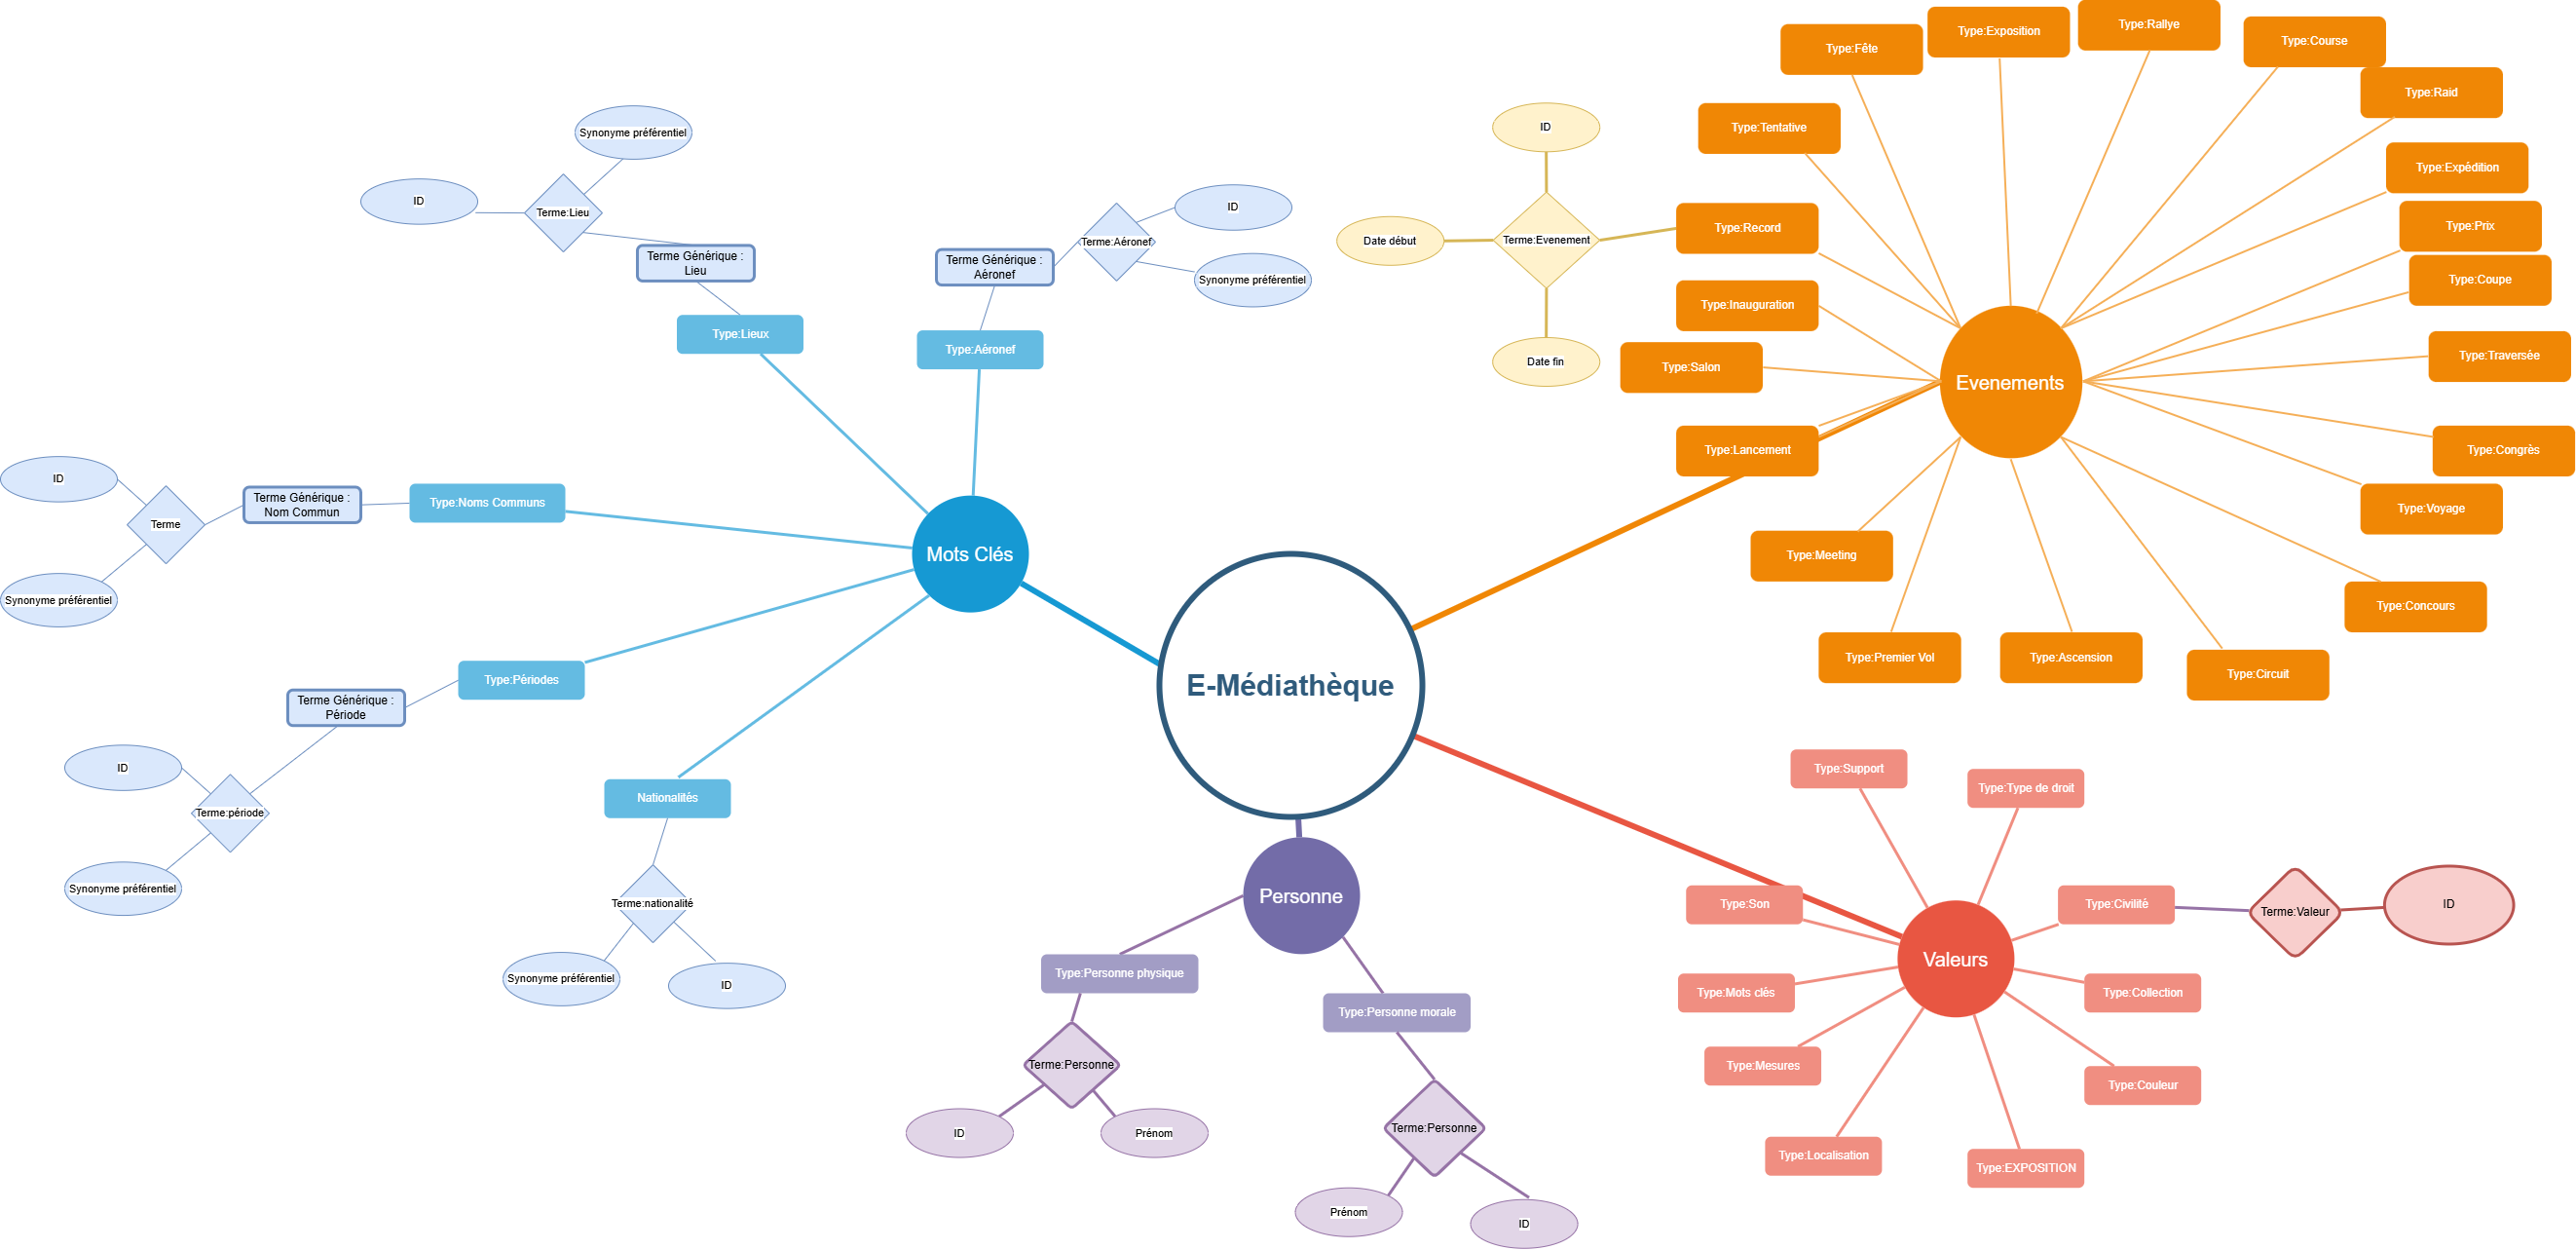
\includegraphics[width=\linewidth]{img/MODEL_emediatheque_mindmap}
		\caption{Modélisation en \textit{mindmap} réalisée avec \textit{draw.io}}
		\label{model:mindmap-emediatheque}
	\end{subfigure}
	\begin{subfigure}{0.35\textwidth}
		\centering
		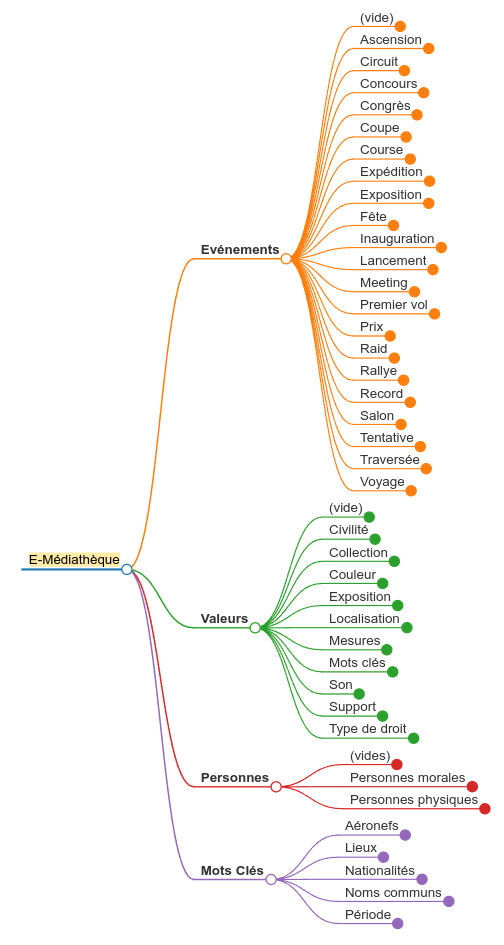
\includegraphics[width=\linewidth]{img/MODEL_emediatheque_arbre}
		\caption{Modélisation en arbre html interactif réalisée avec \textit{markmap}}
		\label{model:arbre-emediatheque}
	\end{subfigure}
	\hfill
	\begin{subfigure}{0.5\textwidth}
		\centering
		\includegraphics[width=\linewidth]{img/GRAPH_emediatheque}
		\caption{Modélisation en graphe réalisée avec \textit{Gephi}}
		\label{model:graph-emediatheque}
	\end{subfigure}
	\caption[Modélisation des \gls{thesaurus} du \mae]{Trois types de modélisations pour un même thésaurus offrent trois approches différentes : notamment, la première permet une vue d'ensemble rapide du type de contenu, la seconde permet d'explorer les branches les unes après les autres, la troisième permet de visualiser des \textit{clusters} de mots -- et pourrait également représenter leurs relations.}
	\label{fig:modelisationthesaurus}
\end{figure}


\paragraph*{Graphes, mindmaps, arbres : l’approche pragmatique}
La visualisation des données par le biais de graphes générés avec Gephi ou d'arbres de concepts interactifs\footnote{Ces arbres, qui auraient également pu être réalisés en Python à l'aide bibliothèques comme \textit{pandas} ou \textit{matplotlib}, ont été réalisés à des fins d'illustration en convertissant un tableau excel en format \textit{markdown} et en générant un fichier html à l'aide de l'application web markmap.} offre une alternative plus intuitive et immédiatement opératoire. Au MAE, ces graphes – qui ont été ensuite mis à disposition de tous les utilisateurs – ont permis de cartographier les clusters thématiques, de détecter les termes orphelins, d'identifier des incohérences dans la hiérarchie des vocabulaires ou des disproportions dans certaines branches du thésaurus. Ils ont servi de support à la restructuration du thésaurus, mais aussi d'outil de médiation entre métiers, lors des groupes de travail ou des ateliers de sensibilisation.

Le format le plus simple -- et donc le plus utilisé, même si moins riche -- a été la modélisation sous forme de \textit{mindmap}, pour représenter seulement les niveaux les plus hauts d'une hiérarchie et travailler sur des grandes catégories de concepts. Celui-ci,  réalisé à partir de logiciels en ligne comme \textit{draw.io}, s'utilise facilement en combinaison avec les tableaux bruts du thésaurus.

On retrouve ici une tension propre à la modélisation documentaire en institution patrimoniale : le compromis entre la formalisation technique – garante de l'interopérabilité et de la pérennité – et la souplesse nécessaire à la prise en main par des agents aux profils variés. Combiner les différents schémas permet ainsi de montrer différents aspects de l'état de l'information au musée, mais aussi de parler à différents profils, et de répondre aux biais, omissions ou transformations inévitables dans toute modélisation et représentation du savoir\footcite{bowkerArrangerChosesConsequences2023}

Ainsi, la modélisation documentaire au \mae~– et plus largement dans les institutions patrimoniales – ne saurait se réduire à un exercice technique. Elle est un instrument de dialogue, d'analyse et de gouvernance, dont la réussite dépend de la capacité à articuler exigence conceptuelle et pragmatisme métier, rigueur des normes et souplesse des usages, pour faire du vocabulaire documentaire un espace partagé, vivant et évolutif.

\begin{table}[htbp]
	\caption{Comparatif des visualisations de données utilisées au MAE pendant le stage}
	\label{tab:comparatif_visualisations}
	\centering
	\setlength{\arrayrulewidth}{0.6pt}
	\renewcommand{\arraystretch}{1.3}
	\begin{tabular}{|p{3cm}|p{4cm}|p{4cm}|p{3cm}|}
		\hline
		\rowcolor{lightgray}
		\textbf{Outil / Visualisation} & \textbf{Avantages principaux} & \textbf{Défauts / Limites} & \textbf{Usages / Destinataires} \\
		\hline
		Diagramme UML & Rigueur, structuration, conformité aux normes (ISO 25964), repérage des écarts avec les standards, interopérabilité forte & Complexité du formalisme, peu accessible pour les non spécialistes, jugé "obscur" & Métiers techniques, experts, audit documentaire \\
		\hline
		Graphe Gephi & Intuitif, interactif, cartographie des clusters, identification des orphelins, support à la restructuration, accessible à tous & Moins formel, difficulté à intégrer des métadonnées complexes, préparation nécessaire & Groupes de travail, ateliers, médiation \\
		\hline
		Arbres de concepts (draw.io, markmap, etc.) & Très accessibles, vues d'ensemble, communication institutionnelle, rapide à réaliser & Peu de granularité, perte de précision sur les liens, adapté aux grandes catégories & Sensibilisation, CA, ateliers \\
		\hline
		Tableaux de synthèse (Excel, markdown) & Utilisation universelle, tri et export rapide, support aux corrections, facile à enrichir & Peu visuel, ne cartographie pas les relations, perte du contexte relationnel & Agents, gestionnaires, formation \\
		\hline
	\end{tabular}
\end{table}

\subsection{La modélisation comme outil de sensibilisation et de pilotage}


La modélisation conceptuelle n’est pas qu’un acte technique : elle est aussi un instrument de sensibilisation et de pilotage institutionnel. Au \mae, l’organisation d’ateliers a permis d’inviter les agents à réfléchir ensemble à la structuration de l’information, à prendre conscience des enjeux de la donnée et de la transmission documentaire.

Ceux-ci ont utilisé la modélisation pour repenser la hiérarchie des termes ou la nomenclature des vocabulaires. Ce travail a permis de concrétiser aux yeux de tous les métiers l'état des connaissances de l'ensemble du musée, et de réfléchir à la manière de les unifier en un unique système.

\bigskip
\bigskip
\bigskip

Ainsi, la modélisation conceptuelle se révèle être le socle sur lequel peut s’édifier une gouvernance documentaire partagée, une culture commune de l’information, et une capacité à piloter le changement dans la durée.

\section{\label{III-A-2}Les solutions techniques existantes : entre standardisation et adaptation locale}


La maîtrise de la prolifération documentaire ne saurait être réduite à une question de modélisation conceptuelle : elle implique le choix raisonné d’outils susceptibles d’articuler la complexité du réel, tout en répondant à des contraintes de gouvernance, d’interopérabilité et de pérennité. Nous nous sommes attachés dans ce mémoire à l'analyse de deux grandes catégories de l'information qui se retrouve dans un musée : celle qui est utilisée pour décrire ses collections, en la matière des thésaurus et vocabulaires contrôlés aujourd'hui présents au musée, et celle qu'il produit quotidiennement dans le cadre de on activité en tant qu'institution publique avec ses archives numériques. Des outils, techniques comme conceptuels, existent pour aider à la structuration et à la diffusion de cette information : nous avons évoqué, pour les archives numérique, l'utilité du respect de normes nationales et d'outils numériques comme une \gls{ged} ou un \ac{sae}. Pour la gestion des vocabulaires contrôlés, c'est un autre outil de modélisation de la connaissance qui s'est imposé : le thésaurus documentaire.



\subsection{\label{III-A-2.1}Qu’est-ce qu’un thésaurus documentaire ?}

On ne peut réduire le thésaurus documentaire à une simple liste de mots ou à un instrument technique. La norme ISO 25964, qui fait aujourd’hui autorité, le définit comme un \enquote{vocabulaire contrôlé et structuré dans lequel les concepts sont représentés par des termes, organisés de façon à ce que des relations entre les concepts soient explicitées, et dont les termes préférentiels sont accompagnés par des entrées vers leurs synonymes ou quasi-synonymes}\footcite{ISO25964120112011,maroyeISO25964Distinction2015}. Celui-ci ne se contente donc pas d’indexer, il articule une vision du monde, une manière de penser le réel à travers le langage documentaire. Il impose donc notamment :
\begin{itemize}
	\item de distinguer le concept (une idée), du terme (le mot choisi pour l'exprimer),
	\item de choisir un terme préféré qui servira à décrire le concept,
	\item de mettre les autres termes en synonymes (\textbf{relations d'équivalence})
	\item des \textbf{relations hiérarchiques} avec :
		\subitem des termes génériques,
		\subitem des termes spécifiques ;
	\item des \textbf{relations d'association} entre les termes,
	\item des définitions, notes et alignements externes associés aux termes.
\end{itemize}

Comme montré dans l'image suivante, la structuration d’un thésaurus suppose ainsi une modélisation précise : chaque concept est relié à des termes, chaque terme préféré est accompagné de notes explicatives, chaque branche de la hiérarchie répond à des logiques de genre à espèce, de tout à partie ou  d'instance à classification\footnote{Pour plus de précisions, consulter l'article suivant \cite{perrinBonnesPratiquesPour2020}}. Cette méthode permet notamment de multiplier les accès à l'information, et de faire entrer en adéquation le langage de l'utilisateur avec le langage de l'institution. 

\begin{figure}
	\centering
	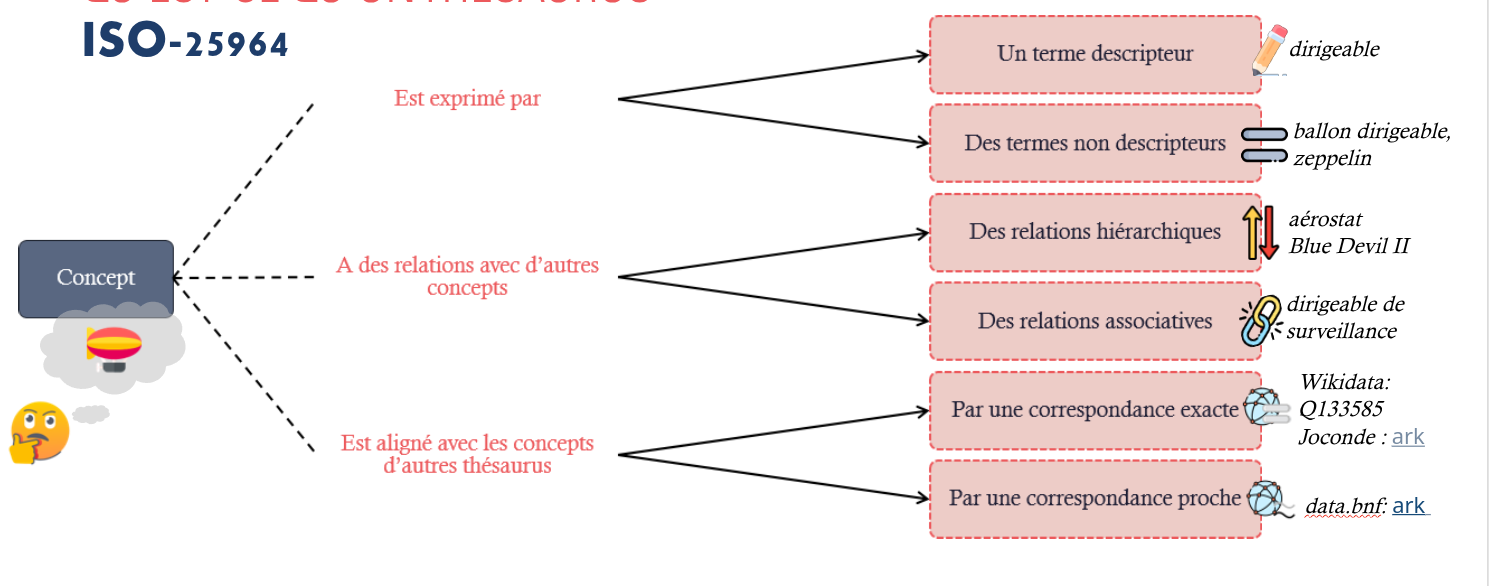
\includegraphics[width=0.9\linewidth]{img/SCHEM_thesaurus}
	\caption[Relations sémantiques exprimées par un thésaurus]{L'ensemble des relations sémantiques exprimées par un thésaurus. \textit{Schéma utilisé dans la formation du 4 juin 2025, inspiré de \protect\cite{perrinBonnesPratiquesPour2020}}.}
	\label{fig:schemthesaurus}
\end{figure}


\subsection{Diversité des outils de structuration de l’information}

Simple et efficace, le \gls{thesaurus} s'est imposé au \mae comme un outil compatible avec les logiciels métiers utilisés. Au fil des réflexions sur leur réorganisation, sont cependant apparues diverses difficultés : il est en effet apparu que le \gls{thesaurus} ne permettrait pas d'englober l'ensemble des connaissances requises au musée pour gérer ses collections. En effet, un thésaurus reste un outil lexical, qui permet de contrôler la description des objets : il ne permet pas, par exemple, de symboliser des liens de famille entre des personnes enregistrées comme terme ou d'expliciter les types de relations -- auteur, constructeur, utilisé dans... -- entre deux termes associés.
Il est apparu que pour arriver à cette granularité d'information, un autre outil devrait être adopté : l'ontologie documentaire. Pour citer Thomas Francart, expert dans les systèmes de gestion des connaissances et fondateur de la société SPARNA, \blockquote{l’ontologie cherche à décrire de façon formelle un domaine de connaissance, en identifiant les types d’objets de ce domaine, leurs propriétés et leurs relations\footcite{francartOntologieThesaurusTaxonomie2013}.}

Bien plus riche que le thésaurus, ce format pourrait répondre aux besoins diversifiés du \mae en lui permettant de couvrir davantage de connaissances, et de mieux adresser la diversité de ses utilisateurs avec un système plus modulables que le thésaurus : sa mise en place demanderait cependant un travail de restructuration, de recherche et de création de liens considérable.

C'est le choix qui a été fait par d'autres institutions devant répondre à des exigences similaires : pour ne pas citer le cas bien connu de la \ac{bnf}, citons par exemple celui de la fondation SAPA -- Archives suisses des arts de la scène qui a migré en 2021 toutes les métadonnées de ses collections en une ontologie utilisant le nouveau standard de description \ac{rdf} \ac{rico}\footnote{Sur \ac{rico}, voir \cite{bruleauxRecordsContextsRIC2024}}. Ce format d'ontologie documentaire lui permet ainsi une granularité extrême et une interopérabilité native avec les standards du web sémantique\footcite{coulonDeploiementNormeRecords2024} : l'auteur insiste cependant sur sa nouveauté, l'absence d'une communauté active pour aider à la mise en place du système, et d'outils informatiques appropriés. Il insiste fortement sur \enquote{le bouleversement de nos pratiques professionnelles qui dépasse la nouvelle norme en elle-même} qu'a apporté la migration, montrant que ce type de projet, bien qu'il aboutisse à un système finalement robuste et efficace pour partager et dépasser les \enquote{silos} de données, demande à l'institution qui le met en place un investissement considérable de temps et de ressources, une familiarisation à ces nouvelles techniques, et exige enfin d'être prêt à changer la manière de travailler de l'ensemble de ses utilisateurs.

\subsection{Solutions pour l’interopérabilité et l’ouverture}

L’histoire des normes documentaires, à ce titre, est celle d’une lente montée en exigence : du premier standard Z39.19, consacré à la structuration des thésaurus pour la recherche documentaire, à la norme ISO 25964 publiée en 2011, qui impose la distinction concept/terme et formalise les relations hiérarchiques, associatives et d’équivalence, chaque étape marque un progrès vers la mise en dialogue des systèmes. Comme le souligne Dominique Chichereau, le mouvement de normalisation des thésaurus qui s'est amorcé dès les années 1970 a accompagné le développement de l’informatisation documentaire , et s’est accéléré avec l’essor du web sémantique et la nécessité d'interopérabilité entre des vocabulaires hétérogènes\footcite{chichereauNormesConceptionGestion2007}.

[TODO : schéma d'explication skos rdf ou ajout au glossaire]
C’est dans ce contexte qu'est apparu \ac{skos}, publié par le \ac{w3c} pour \enquote{proposer un système permettant d’exprimer et de gérer des modèles interprétables par les machines dans la perspective du web sémantique\footcite{lenartSKOSLangageRepresentation2007}}, en offrant un modèle fondé sur des triplets \ac{rdf}. Ce standard permet notamment de décrire les concepts, leurs labels multilingues, et les relations hiérarchiques ou associatives entre eux.  \ac{skos} s’impose dès lors comme un langage technique idéal,\enquote{défini comme « simple » par opposition à d’autres modèles, comme OWL (Ontologic Web Language)}, pour mutualiser les vocabulaires sur le web tout en respectant la complexité des relations et la richesse des annotations. 

Bien qu'il existe d'autres solutions de gestion du vocabulaire et que l'avènement de l'intelligence artificielle pousse des institutions à se tourner vers des modèles plus complexes pour implémenter des solutions IA, de la Bibliothèque nationale de Finlande, qui expose ses vocabulaires sur Skosmos\footcite{Skosmos} également utilisé pour le thésaurus de l’UNESCO\footcite{unescoThesaurusLUNESCO1977}, en passant par des institutions patrimoniales françaises telles que le ministère de la Culture avec le thésaurus de Joconde\footcite{ministeredelacultureListeDautoriteDenomination} ou le réseau \ac{frantiq}\footcite{Pactols}, l’usage du format \ac{skos} pour la structuration et la diffusion de thésaurus s’est aujourd’hui imposé aussi bien dans le monde de la recherche, de l’administration publique que dans l’écosystème documentaire des grands musées.
	
	
L’avènement de \ac{skos} et la généralisation du web sémantique n’ont pas seulement permis d’exposer les vocabulaires : ils ont ouvert la voie à une ambition nouvelle, celle de l’alignement des données, qui consacre la possibilité pour chaque institution de faire dialoguer ses savoirs avec ceux de ses pairs. Aligner en effet, c'est relier explicitement des concepts équivalents ou proches, structurer leurs correspondances à l’aide des propriétés (en \ac{skos}, \lstinline|skos:exactMatch|, \lstinline|closeMatch|, \lstinline|broadMatch| ou \lstinline|related|). Ce travail, loin d’être purement technique, engage une réflexion sur la valeur des termes, la portée des synonymes et la fidélité aux usages locaux : il impose de choisir, parmi la profusion des vocabulaires, ceux qui feront pont entre les systèmes et permettront la circulation des connaissances. Au \mae -- ou il n'est encore qu'à l'état de projet -- comme ailleurs, l’alignement avec les thésaurus de Joconde, le SUDOC ou Wikidata ne se réduit pas à un échange de fichiers : il suppose une révision minutieuse des branches, une concertation des acteurs, une vigilance sur les notes historiques et les spécificités des collections. Cette opération apparaît ainsi comme le prolongement naturel de toute politique documentaire soucieuse d’ouverture et de pérennité, pour garantir à l'institution sa capacité à se transmettre, à s’enrichir, et à dialoguer au sein d’un univers patrimonial interconnecté.

\section{\label{III-A-3}L’intégration dans l’écosystème institutionnel : vers une gouvernance collaborative des outils}

L’intégration du logiciel Opentheso au \mae~semblerait être la solution qui réponde le mieux à ses aspirations de gouvernance du vocabulaire et d'interopérabilité avec le web. Cet outil libre recommandé par le ministère de la Culture, s’impose aujourd'hui en France comme le socle d’un vocabulaire  capable de transcender les cloisonnements logiciels et de fédérer les métiers. Sa conformité aux normes ISO 25964 et au standard \gls{skos}, sa capacité à exporter dans des formats interopérables \gls{rdf}, comme \textit{Turtle} ou \textit{JSON-LD}, à visualiser l’arborescence en graphe, à documenter les relations synonymiques ou hiérarchiques, en font un instrument rigoureux qui peut être au service à la fois de la recherche et de la médiation. Opentheso permet de structurer la connaissance, mais aussi de relier les bases métiers – un plugin d'intégration dans \gls{koha} existe déjà, et il serait envisageable de demander une intégration à \textit{Skinsoft} pour Archange qui permettrait au logiciel d'interagir avec l'\ac{api} d'OpenTheso.

La mise en place, en complément, d'un réseau de logiciels dédiés à une gestion rationalisée de l'information au \mae~-- comme des versements réguliers sur le \gls{sae} Vitam pour l’archivage et la mise en place d'une \gls{ged} – serait d'une grande aide au musée pour parvenir à ses ambitions de gouvernance.

\subsection{Accompagnement au changement et formation des agents}

Toute réforme documentaire ne pourra cependant aboutir sans accompagnement au changement : ateliers de sensibilisation, guides d’usage, fresques de la connaissance, tutoriels, autant de dispositifs qui harmoniseraient les pratiques et préparent les agents à la prise en main des nouveaux outils. La formation s'imposera comme la condition de la réussite : elle permettra de comprendre la logique des outils, de s’approprier les méthodes de structuration et d’assurer la pérennité des acquis.

\subsection{Interopérabilité et dialogue intermétiers}

L’interopérabilité enfin, même si la mise en place de solutions dédiées l'aidera grandement, ne se limitera pas à la technique : elle suppose un dialogue continu entre les métiers du musée et une construction de passerelles entre les silos professionnels et plateformes. Les groupes de travail menés au musée ont permis de réfléchir à des solutions communes pour l’archivage numérique et l'unification des thésaurus, ils devront continuer pour les mettre en place et assurer leur bon fonctionnement. 


\bigskip
\bigskip
\bigskip

\lettrine{A}insi se dessine, à travers l’expérience du Musée de l’Air et de l’Espace, une voie exigeante pour la maîtrise de la prolifération documentaire. Il ne s’agit pas seulement de juxtaposer modèles conceptuels, outils techniques et dispositifs de gouvernance : il faut les articuler, les penser ensemble, dans une logique de préservation de la richesse sémantique et d’ouverture à l’interopérabilité. Les solutions expérimentées — modélisation via Gephi, migration vers Opentheso, ateliers de sensibilisation, harmonisation documentaire — illustrent la nécessité d’allier rigueur, adaptation et accompagnement au changement pour garantir la transmission du patrimoine et la vitalité de l’écosystème muséal.
	\chapter[Gérer la prolifération]{\label{III-B} L'unification des thésaurus : un processus collaboratif}



\lettrine{I}ntro

\section[Un processus collaboratif]{\label{III-B-1}Convaincre de la nécessité du processus}

La structuration du savoir, loin d’être un acte isolé, engage l’institution dans une négociation permanente entre ses acteurs, ses usages et ses impératifs de transmission. La mise en œuvre d’une unification des thésaurus au sein du \mae~ne procède donc pas d’une simple injonction technique. Comme nous l'avons vu précédemment, bibliothèque, e-médiathèque et musée disposent chacun de leurs référentiels propres, hérités d’usages, de logiques métiers et de logiciels distincts. Le \mae~étant intégré au réseau des musées et bibliothèques du \minarm, toute décision d’unification --- à titre d’exemple, l’intégration d’OpenTheso dans \gls{koha}\footnote{Cette intégration est possible grâce à un plugin développé par la société \textit{Tamil}, voir \cite{PluginTamilOpentheso}} --- peut posséder un impact qui dépasse le seul cadre du \mae~pour concerner l'ensemble de ces institutions. Il est donc illusoire de prétendre harmoniser localement une pratique documentaire sans se heurter à la doctrine technique et documentaire imposée à l’échelle ministérielle : ceci rend la négociation indispensable.

Or, nous avons vu que l’interopérabilité s’impose comme une condition de la communicabilité et de la valeur scientifique du fonds documentaire\footcite{hudonISO25964Pour2012a, maroyeISO25964Distinction2015}. Convaincre de la nécessité du processus, c’est inscrire la démarche dans une logique de mutualisation, de visibilité accrue des collections et de conformité aux standards nationaux et internationaux (ISO 25964, \gls{skos}).

\paragraph*{Solution proposée au \mae}
Mais ce chantier excède de loin le quotidien des usagers du thésaurus. L’unification s’ajoute aux missions ordinaires des agents, requérant du temps, des compétences techniques et une acculturation documentaire spécifique. La réussite du processus dépend en effet de l’implication des agents, des groupes de travail transversaux, du partage de la documentation et de la prise en compte des besoins spécifiques de chaque métier. Insister sur la dimension collaborative est essentiel : seule la concertation régulière entre les différents usagers des thésaurus permet de dépasser les clivages métier. Cette sensibilisation s'est faite au \mae via une brève formation de sensibilisation des agents du \ac{dsc} au sujet des \gls{thesaurus} en général, et à ceux du musée en particulier. Des courts ateliers pratiques et l'implication des agents dans divers groupes de travail ont ainsi permis de lancer le processus et de montrer par la pratique les enjeux de cette unification et la méthode à poursuivre.

\section{\label{III-B-2}Créer un thésaurus commun à partir des vocabulaires existants : un travail collaboratif}

L’unification procède d’une méthodologie précise : la démarche adoptée au musée s’est articulée autour d’une formation initiale sur ce qu’est un thésaurus, suivie par des groupes de travail généraux pour explorer l'ensemble des thésaurus et recueillir les usages de chacun pour dégrossir les besoins, puis par des groupes thématiques qui ont examiné chaque type de branche (mots-clés, constructeurs, événements, périodes, matériaux...). Selon le corpus, deux approches se sont dégagées : 
\begin{itemize}
	\item soit une analyse terme à terme lorsque le corpus était limité (définition, synonymes, organisation hiérarchique à partir du niveau haut),
	\item soit une recherche de niveaux hauts communs, puis le rangement progressif des termes spécifiques par la suite.
\end{itemize}
À chaque étape, il a fallu observer les règles de normalisations qui avaient pu être suivies dans le passé et proposer des pistes pour en définir de nouvelles qui puissent être générales au musée.

L’harmonisation des branches et des hiérarchies se fait progressivement, en s’appuyant sur les recommandations institutionnelles (Ministère de la Culture, Joconde\footnote{Voir \cite{ministeredelacultureVocabulairesScientifiquesService2014}} pour le musée). Elle est loin d'être achevée aujourd'hui, mais les premières bases ont été posées pour continuer ce travail d'unification et migrer --- à une date qui n'est pas encore définie et qui sera à négocier avec la tutelle --- vers une plateforme de gestion comme OpenTheso\footcite{OpenThesoa} qui permette de faciliter la maintenance de ce travail.

Le processus de fusion, enfin, s’est construit sur la base des vocabulaires existants : il a fallu croiser les listes de termes, identifier des synonymes et des concepts communs, avant de constituer un référentiel central validé collectivement et partagé sur SharePoint.

\subsection{La réflexion en groupes de travail : avantages et limites}

Le travail collectif a présenté des avantages incontestables : il a notamment permis de mutualiser l'expertise de chacun, de confronter les usages et les logiques métiers et de discuter de solutions pragmatiques qui conviennent à l'ensemble des usagers --- c'est par exemple lors de ces réunions qu'il a été choisi de garder au singulier les mots-clés du thésaurus, de les écrire en minuscules contrairement à ce qui était en usage à la bibliothèque, ou ce qui a permis de relever les difficultés inhérentes à la dénomination et à la hiérarchisation des constructeurs d'avions, dont l'histoire mouvementée rend toute classification difficile.

Mais ce mode de travail comporte aussi de réelles limites : le thésaurus étant un outil de structuration du vocabulaire, il reste nécessaire de se pencher sur l'ensemble des mots qu'il contient pour les organiser et les définir. Or, le volume de données à traiter est considérable et il s'est avéré que ce mode de travail ne serait pas suffisant pour l'unification des thésaurus, et qu'une personne seule, ou un groupe de trois personnes maximum peut être plus efficace --- en s'attelant à un travail de tri au fur et à mesure, par petites séances --- qu'un groupe dont l'objectif sera plutôt de discuter des modifications que de les appliquer. Dans l'un ou l'autre cas cependant, la clé d'une harmonisation efficace reste la communication : toute modification doit être explicitée et confrontée au point de vue des autres métiers avant d'entrer en vigueur.

\inserttable{img/TABL_cr_gt_thematique}

\subsection{Où se situent les principaux besoins ?}

Le constat est paradoxal : ce n’est pas dans les segments les plus techniques ou spécialisés que le besoin d’unification se fait le plus sentir --- par exemple, les \gls{thesaurus} des constructeurs d'avions des trois instances sont déjà structurés, et s'il est nécessaire de définir des normes d'écriture et d'expliciter la méthodologie de hiérarchisation, ils restent sensiblement proches. Ces vocabulaires en effet sont déjà travaillés, et adossés à la physicalité des objets ou des institutions qu'ils décrivent. 

Les difficultés majeures surgissent dans les intersections avec les autres institutions patrimoniales, là où le choix entre le respect des normes (ISO 25964, Joconde, \ac{sudoc}) et la conservation des spécificités du musée devient le plus épineux : il en a été ainsi pour le thésaurus des matériaux utilisés principalement pour la description des collections : sa réorganisation et sa reconstitution ont demandé un travail considérable de recherche de définitions et de consultation de ce qui était fait sur Joconde pour arriver à un résultat proche des recommandations du ministère de la Culture.

\bigskip
\bigskip
\bigskip

\lettrine{I}ci conclusion
	\chapter[Apports de l'\ac{ia}]{\label{III-C}L'IA : une aide devant la masse des données ?}

\lettrine{L}a croissance exponentielle des données numériques au sein des institutions patrimoniales -- thésaurus, notices, archives, corpus iconographiques -- fait émerger un constat d’impuissance : l’humain semble ne pas suffire pour garantir leur intégrité et leur bonne organisation. Au \mae, la réorganisation et l'harmonisation des vocabulaires, l’identification des doublons, la création de relations d'associations et l'ajout de définitions aux termes mobilisent des volumes de données qui excèdent largement la capacité de traitement manuel des agents. Ces tâches chronophages de comparaison et d'enrichissement des thésaurus et d'autres tâches de la vie quotidienne du musée comme l'indexation et la correction de notices ont amené la question de l'usage de l'intelligence artificielle comme aide pour l'agent. Lors de notre stage, nous avons pu ainsi explorer quelques pistes d'utilisation de l'\ac{ia}, sans toutefois aller plus loin dans l'implémentation de ses solutions -- en effet, ce projet ne rentrant pas dans le périmètre direct des missions du stage, il a été choisi de se concentrer davantage sur la constitution d'une base de vocabulaire aéronautique de référence à partir de \textit{Wikidata}. Avant de détailler les solutions proposées, leurs perspectives et leurs limites, nous nous pencherons brièvement sur les réalités de l'utilisation de l'\ac{ia} en institution patrimoniale.  


%%%%%%%%%%%%%


\section{\label{III-C-1}Automatiser les tâches : promesses et réalités de l’IA en institution patrimoniale}

La croissance exponentielle des données numériques au sein des institutions patrimoniales -- thésaurus, notices, archives, corpus iconographiques -- fait émerger un constat d’impuissance : l’humain semble ne pas suffire pour garantir leur intégrité et leur bonne organisation. Au \mae, la gestion quotidienne des vocabulaires, l’identification des doublons, la création de relations d'associations et l'ajout de définition aux termes mobilisent des volumes de données qui excèdent largement la capacité de traitement manuel des agents. Ces tâches chronophages de comparaison et d'enrichissement des thésaurus et d'autres tâches de la vie quotidienne du musée comme l'indexation et la correction de notices, amènent la question de l'usage de l'intelligence artificielle comme aide pour l'agent.

Face à cette surcharge, elle semble en effet promettre un grand allègement : comme d'autres projets l'ont montré, celui ci n'est efficace que dans la mesure où l'équilibre avec l'expertise humaine est respecté. \enquote{L’\ac{ia} est \textelp{} un outil complémentaire qui, bien encadré, permettrait d’assister les équipes sans remettre en cause l’expertise humaine essentielle à la validation des informations\footcite{bermesRepenserCollectionsPatrimoniales2025}.} Les cas d’utilisation se multiplient dans les institutions patrimoniales, principalement pour l’indexation automatique : on peut citer par exemple le projet d'indexation automatique RAMEAU à la \ac{bnf} \footcite{filabesLindexationRAMEAUAssistee2025}, ou TORNE-H\footcite{bermesRepenserCollectionsPatrimoniales2025} au Musée des arts décoratifs. Les modèles de langage y assistent la reconnaissance des entités, l’extraction et la normalisation des termes. Les méthodes d’apprentissage supervisé permettent désormais de nettoyer les vocabulaires, de regrouper les variantes et d’automatiser la détection d’incohérences (que ce soit avec l'assistance de \textit{LLM} ou de bibliothèques Python comme \textit{NLTK} ou \textit{spaCy}, distances de chaînes comme \textit{Levenshtein}, modèles linguistiques type \textit{CamemBERT} ou \textit{sentence-transformers}) :

\inserttable{img/TABL_outils_ia.tex}

Ces outils efficaces semblent pour l'instant rester cantonnés à des projets pilotes ou à des institutions prestigieuses dont les ressources sont plus élevées que celles du \mae. Le passage de l’expérimentation à la routine semble, pour l’heure, demeurer l’exception dans la majorité des institutions patrimoniales.

\section{\label{III-C-2}Entraîner une IA sur la base d’un vocabulaire spécialisé : défis et solutions}

Cette ambition d’automatiser le traitement des thésaurus se heurte, au MAE, à des contraintes majeures. Ce musée, sous tutelle du \minarm, ne saurait exposer ses données sensibles -- notices techniques, archives, référentiels -- à des modèles externes ou à des services cloud\footnote{A ce sujet, les support informatique du musée se conforme autant que possible aux recommandations de l'\ac{anssi}, et à la suite des méfiances exprimées par l'organisme concernant la sécurité et la confidentialité des données d'entraînement des \ac{llm}, la nouvelle charte informatique de septembre 2025 demandera à tous les agents de s'engager à ne pas les utiliser.}. La confidentialité, renforcée par le \ac{rgpd} et les restrictions propres au secteur, impose une politique de sécurité stricte : tout entraînement doit s’effectuer sur des outils déployés en interne, sur serveurs sécurisés, sans échange hors du périmètre institutionnel.

La méthodologie proposée lors de ce stage pour entraîner une IA sur les vocabulaires spécialisés du musée tente de faire face à ces contraintes. L’entraînement à partir de Wikidata, par extraction du vocabulaire aéronautique via requêtes SPARQL\footnote{Cf. [TODO annexe]}, permet de sélectionner des concepts pertinents, mais génère un bruit considérable : l'exhaustivité reste partielle, et il est difficile de ne pas récupérer de termes non pertinents ce qui nécessite un nettoyage manuel important.

Une autres difficulté rencontrée est le manque de précédent sur des projets de ce type : si les projets d'implémentation de l'\ac{ia} pour des tâches d'indexation -- où celle-ci peut donc mettre chaque oeuvre dans un contexte, de contenu ou de description --, aucun précédent d'utilisation pour traiter un thésaurus semble n'avoir été réalisé, ou du moins diffusé sur le web. La tâche est en effet complexe : dans un thésaurus, chaque mot est indépendant, et il comprend peu de matière de contextualisation dont un modèle de type \textit{bert}\footnote{voir paragraphe précédent} aurait besoin. La solution semble donc être l'utilisation d'un \ac{llm} : cependant, ceux-ci peinent à saisir les nuances du vocabulaire extrêmement spécialisé utilisé par le musée. La solution qui a donc été proposée est l'entraînement d'un \ac{llm} en local\footnote{des tests encore peu concluant ont été réalisés avec le modèle \textit{llama3:2}} sur les données extraites de Wikidata -- dont les termes sont déjà définis et associés entre eux -- et un corpus de données du musée avant de lui fournir les fichiers csv des thésaurus du musée pour lui demander de reconnaître d'éventuels synonymes, associations, et hiérarchisations\footnote{[TODO : ajout annexe prompt et modèle]}. 

\subsection{Limites et perspectives}

À ce stade cependant, demeure la limite de la spécialisation du vocabulaire du musée : même si l'\ac{ia} peut permettre d'alléger la charge de travail des agents travaillant à l'unification du thésaurus, une validation humaine reste nécessaire, pour entraîner l'\ac{ia} et valider ses données. Ceci demande donc de mettre en place une pratique hybride qui articulerait automatisation et savoir-faire documentaire, avant d'aligner le résultat sur des formats \ac{skos}/\ac{rdf}, dans le respect des contraintes propres au musée.

La réflexion sur l’apport de l’IA en institution patrimoniale ne se résume pas à une question d’outillage : elle engage en effet un débat sur la gouvernance de l’information et sur la capacité de l’institution à transmettre son patrimoine sans le dissoudre dans l’automatisme. L'\ac{ia}, ici comme ailleurs, ne reste utile que si elle demeure un auxiliaire du métier et non un substitut. 

\bigskip
\bigskip
\bigskip

%\lettrine{I}ci conclusion
	
	%%%%%%%%%%%%%%%%%%%%%%%%%%% CONCLUSION %%%%%%%%%%%%%%%%%%%%%%%%%%%
	
	Ici, je pourrai mettre la conclusion de cette partie
	
	%%%%%%%%%%%%%%%%%%%%%%%%%%%%%%%%%%%%%%%%%%%%%%%%%%%%%%%%%%%%%%%%%%
	%%%%%%%%%%%%%%%%%%%%%%%%%%% CONCLUSION %%%%%%%%%%%%%%%%%%%%%%%%%%%
	%%%%%%%%%%%%%%%%%%%%%%%%%%%%%%%%%%%%%%%%%%%%%%%%%%%%%%%%%%%%%%%%%%
	
	\chapter*{Conclusion}
	\addcontentsline{toc}{chapter}{Conclusion}
	\newpage{\pagestyle{empty}\cleardoublepage}
	
	
	
	
	
	
	
	%%%%%%%%%%%%%%%%%%%%%%%%%%%%%%%%%%%%%%%%%%%%%%%%%%%%%%%%%%%%%%%%%%
	%%%%%%%%%%%%%%%%%%%%%%%%%% BACKMATTER %%%%%%%%%%%%%%%%%%%%%%%%%%%%
	%%%%%%%%%%%%%%%%%%%%%%%%%%%%%%%%%%%%%%%%%%%%%%%%%%%%%%%%%%%%%%%%%%
	
	%%%%%%%%%%%%%%%%%%%%%%%%% ANNEXES %%%%%%%%%%%%%%%%%%%%%%%%%%%%%%%%
	%%%%%%%%%%%%%%%%%%%%%%%%%%%%%%%%%%%%%%%%%%%%%%%%%%%%%%%%%%%%%%%%%%
	
	\appendix %Des appendices: tables figures, etc
	
	%%%%%%%%%%%%%%%%%%%%%%%%%%% ANNEXE 1 %%%%%%%%%%%%%%%%%%%%%%%%%%%%%
	\part*{Annexes}
	\addcontentsline{toc}{part}{Annexes}
	
	\chapter[Chronologie du MAE]{\label{Ax-A}Chronologie du \mae}
	\LTXtable{\textwidth}{./parties/backmatter/annexes/A1_frise.tex}
	
	\chapter[Organigramme]{\label{Ax-B}Organigramme du \mae}
	\begin{figure}[htbp]
		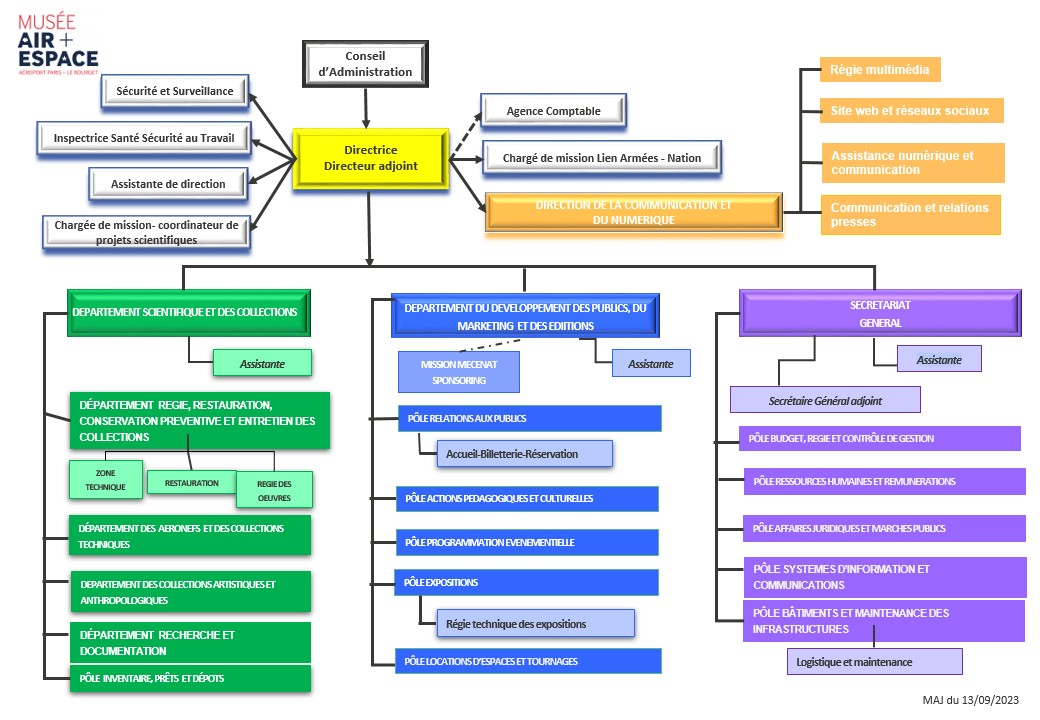
\includegraphics[width=\linewidth]{img/SCHEM_organigramme.jpg}
		\label{fig:schem_organigramme}
	\end{figure}
	
	\chapter[Flux de données]{\label{Ax-C}Flux de données de thésaurus au \mae}
	\begin{figure}[htbp]
		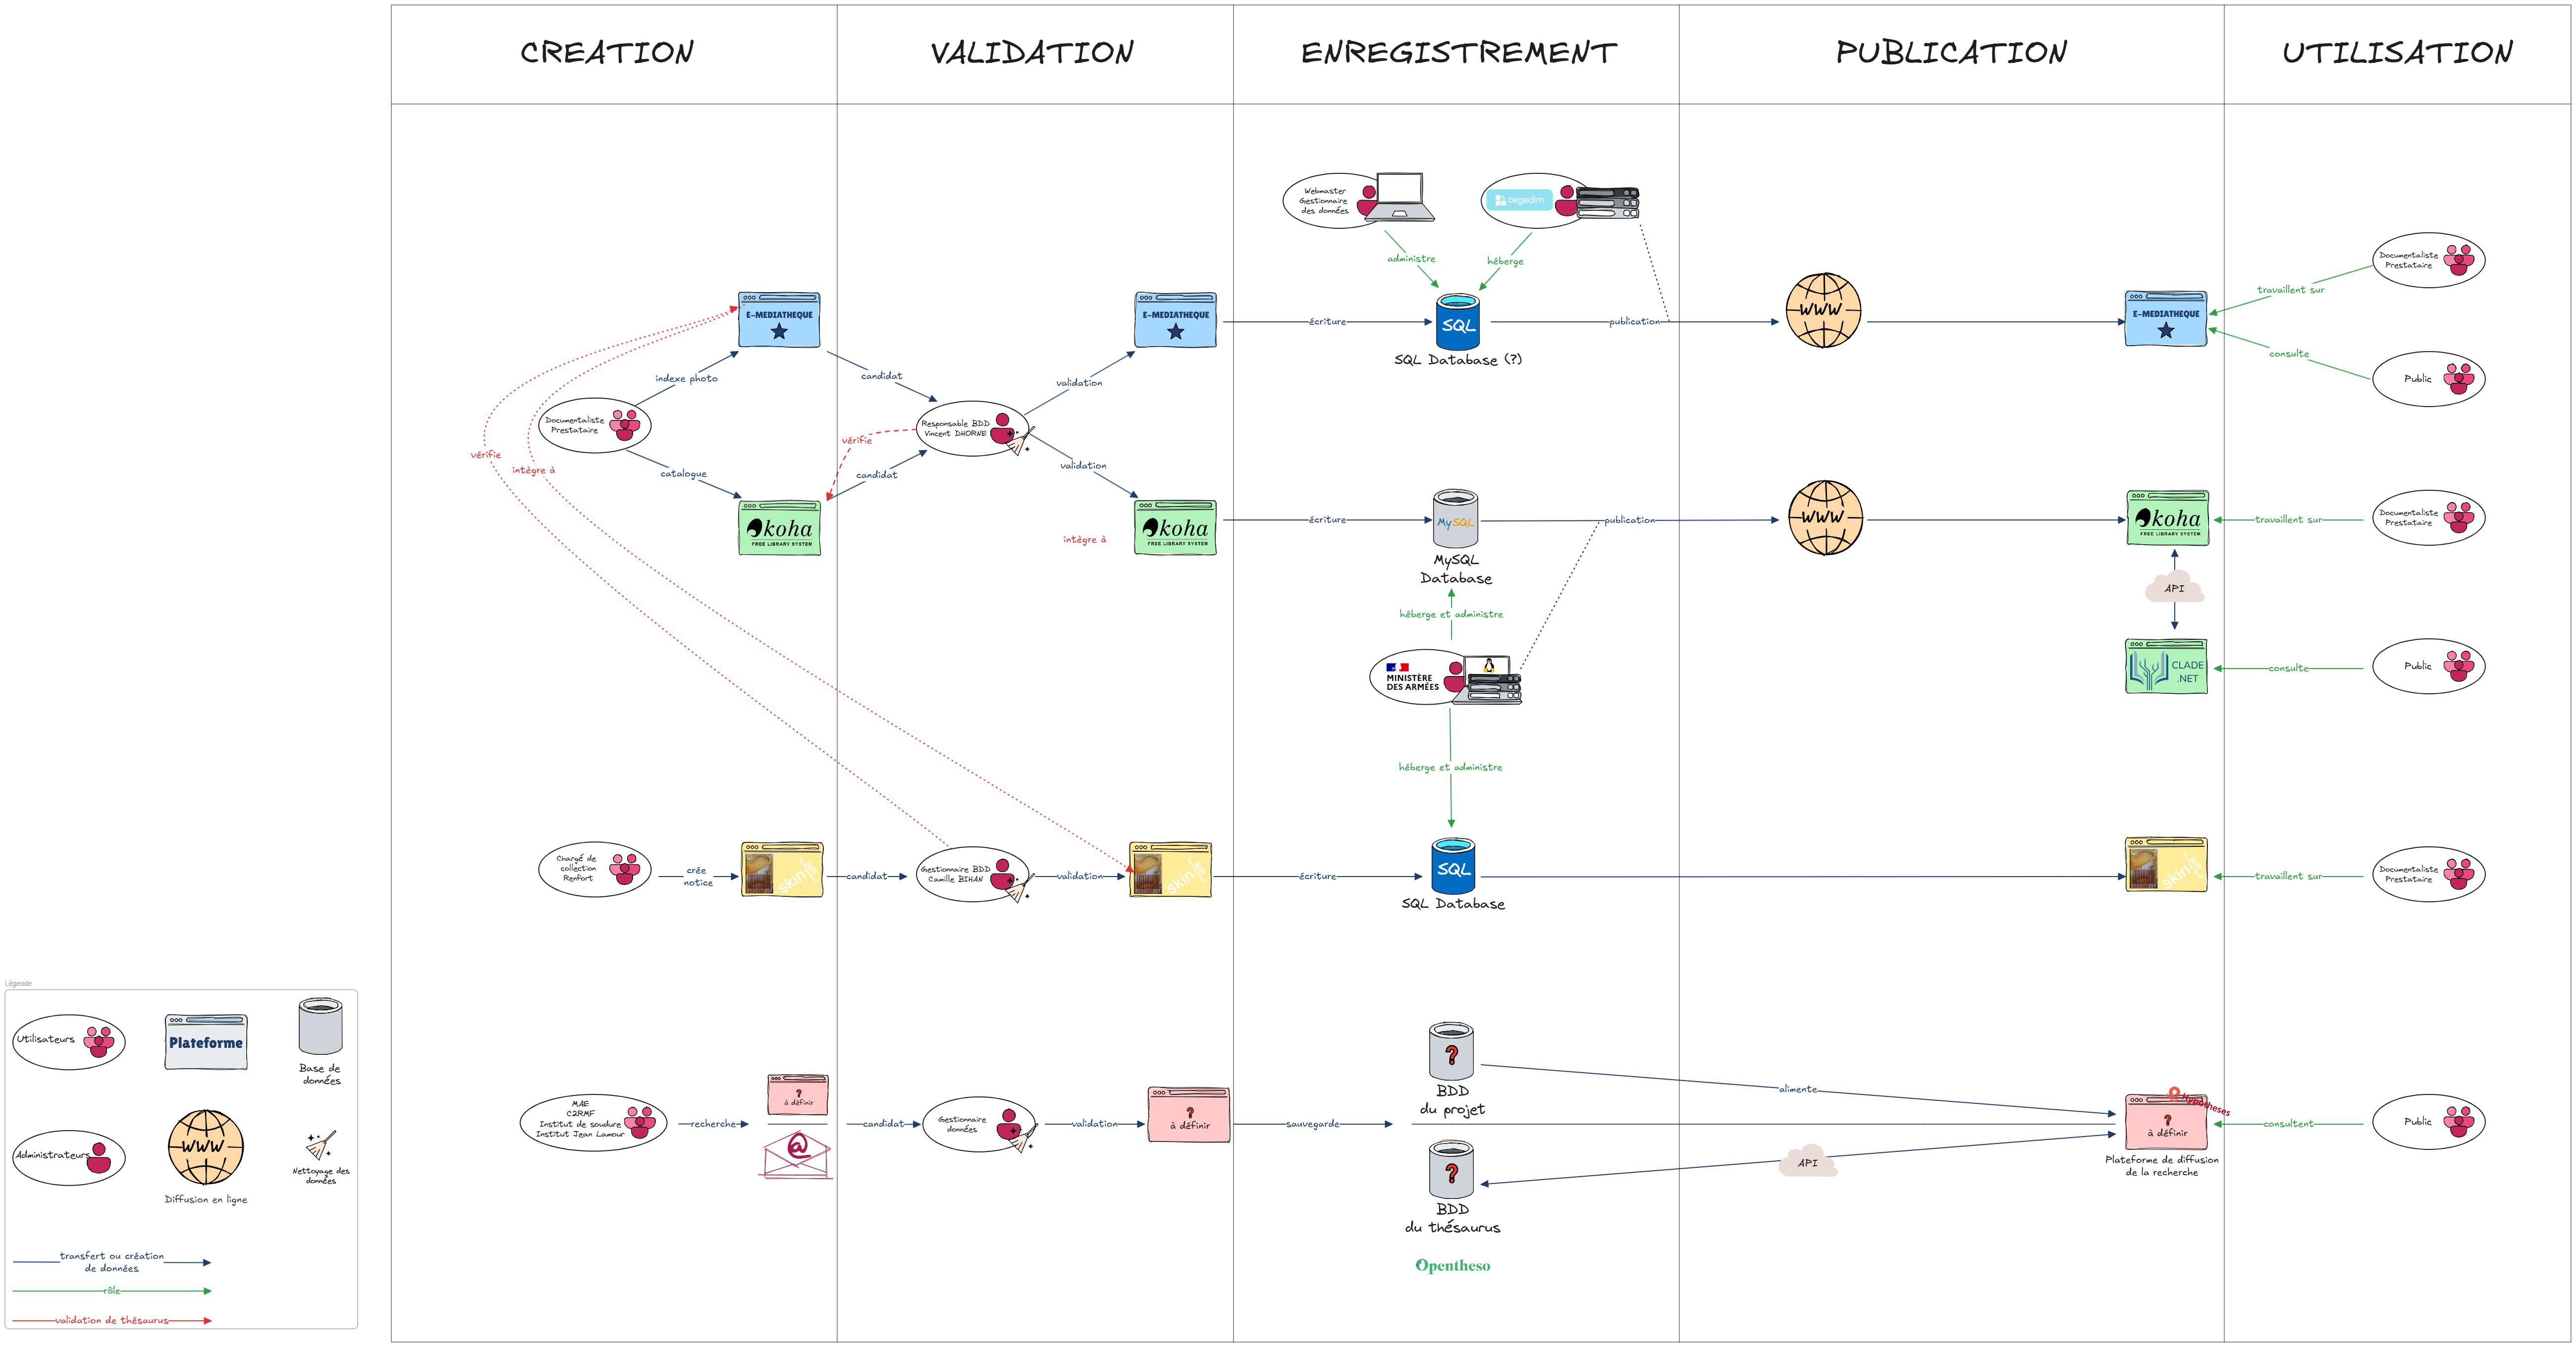
\includegraphics[width=\textwidth]{img/MODEL_Flux.png}
		\label{fig:model_flux}
	\end{figure}
	
	\chapter[Interview V. Dhorne]{\label{Ax-D}Interview de Vincent Dhorne, documentaliste au \mae (20 mai 2025)}
	%%%%%%%%%%%%%%%%%%%%%%%%%%%%%%%%%%%%%%%%%%%%%%%%%%%%%%%%%%%%%%%%%%%%
%%%%%%%%%%%%%%%%%%%%%%% ANNEXE - INTERVIEWS %%%%%%%%%%%%%%%%%%%%%%
%%%%%%%%%%%%%%%%%%%%%%%%%%%%%%%%%%%%%%%%%%%%%%%%%%%%%%%%%%%%%%%%%%%%
\section*{Entretiens avec les professionnels}

\subsection*{Entretien avec Vincent Dhorne, documentaliste}
\subsection{A FAIRE VALIDER PAR VINCENT}

\textit{Entretien réalisé le 20 mai 2025}
\indent Présents : \textit{Maëlys Gioan, Vincent Dhorne}

\subsubsection*{La bibliothèque et ses thésaurus}

\question{Le fichier que j'ai en ma possession comprend-il l'ensemble des données du thésaurus de la bibliothèque ? N'y a-t-il pas de définitions supplémentaires, de langues différentes, etc. ?}

\reponse{Oui, le fichier est complet. Il n'y a pas d'éléments supplémentaires.}

\question{Lorsque le thésaurus a été conçu, une structure particulière a-t-elle été suivie ? Comment décidiez-vous qu'un terme devait être en descripteur principal plutôt que terme générique d'un descripteur plus spécifique ?}

\reponse{[Cette question n'a pas reçu de réponse précise lors de l'entretien]}

\question{Quelles seront les applications utilisées par les agents et par les utilisateurs après la migration ?}

\reponse{Koha pour la gestion et Clade pour la diffusion.}

\question{Selon vous, qui est compétent dans le service pour le thésaurus ? Quelles sont les spécificités du thésaurus de la bibliothèque par rapport aux autres ?}

\reponse{C'est moi qui m'en occupe. Notre thésaurus est peut-être plus intéressant pour les avions récents.}

\question{D'où viennent les données des thésaurus ? Qui les saisit ? Qui les valide ?}

\reponse{Les documentalistes font des propositions de candidats en cataloguant, c'est moi qui m'occupe de les valider pour les intégrer au thésaurus.}


\subsubsection*{L'e-médiathèque}

\question{Qu'est-ce qui relève du thésaurus à proprement parler, et qu'est-ce qui relève plutôt de la normalisation de l'indexation ?}

\reponse{Ce qui constitue les mots clés (lieux, aéronefs...) constituent le thésaurus. Les personnes, événements et valeurs ne sont pas des thésaurus à proprement parler et plutôt des listes contrôlées.}

\question{Sur quoi ce thésaurus fait-il autorité ?}

\reponse{Selon [la gestionnaire de base de données], sur les constructeurs. Pour ma part, je ne vois pas d'interaction avec les autres thésaurus.}

\question{N'y aurait-il pas des données qui gagneraient à être récupérées depuis d'autres référentiels ? Par exemple pour les valeurs ou les lieux, et ne garder que les termes propres au musée à gérer ?}

\reponse{Pour les lieux, ce serait possible. Pour les autres éléments, c'est trop spécifique au musée.}

\question{D'où viennent les données des thésaurus ? Qui les saisit ? Qui les valide ?}

\reponse{[Un documentaliste] fait des ajouts en tant que candidat, puis je valide et j'ajoute. Pour les avions, je vérifie par rapport aux ouvrages de référence.}

\question{Où sont-elles hébergées ?}

\reponse{Le prestataire Cegedim stocke les données. Une autre prestation assure la maintenance de la base et du logiciel de l'e-médiathèque.}

\subsubsection*{Historique des thésaurus}

\question{Quand chaque thésaurus a-t-il été créé, approximativement ?}

\reponse{Alexandrie date de 1994. Pour Micromusée, il y a eu des réunions thésaurus vers 2000 avec les documentalistes lors de l'import des photos. Des ajouts ont été faits au fur et à mesure par les chargés de collections selon leurs besoins, jusqu'en 2016 pour la fin des photos.}

\question{Aujourd'hui, quels sont les liens entre les thésaurus ? Y a-t-il des interactions pour demander quel terme utiliser ?}

\reponse{Aucune interaction, sauf peut-être une vérification dans Alexandrie avant de créer un terme dans l'e-médiathèque. Depuis au moins le Covid où nous n'avions plus accès au serveur de Micromusée, l'habitude de vérifier les données avant de les ajouter aux thésaurus du DRD s'est perdue.}

\subsubsection*{Observations complémentaires}

Lors de cet entretien, plusieurs éléments ont été clarifiés concernant l'organisation des données :
\begin{itemize}
	\item Une vérification sur Alexandrie est parfois effectuée avant l'ajout d'un nouveau terme, surtout pour l'aviation moderne
	\item L'aviation ancienne est plutôt vérifiée sur Micromusée
	\item Pendant le confinement, l'accès à distance à Micromusée n'était pas possible ce qui a contribué à la séparation des ensembles de thésaurus
\end{itemize}	
	\newpage{\pagestyle{empty}\cleardoublepage}
	
	
	
	\backmatter % glossaire, index, table des figures, table des matières.. (la bibliographie a déjà été appelée)
	
	%%%%%%%%%%%%%%%%%%%%%%%%%%%%%% INDEX %%%%%%%%%%%%%%%%%%%%%%%%%%%%%
	%%%%%%%%%%%%%%%%%%%%%%%%%%%%%%%%%%%%%%%%%%%%%%%%%%%%%%%%%%%%%%%%%%
	
	%\printindex
	
	%%%%%%%%%%%%%%%%%%%%%%%%%%% GLOSSAIRE %%%%%%%%%%%%%%%%%%%%%%%%%%%%
	%%%%%%%%%%%%%%%%%%%%%%%%%%%%%%%%%%%%%%%%%%%%%%%%%%%%%%%%%%%%%%%%%%
	
	\printglossaries
	\addcontentsline{toc}{part}{Glossaire}
	
	%%%%%%%%%%%%%%%%%%%%%%%%%% TABLES DES MATIÈRES %%%%%%%%%%%%%%%%%%%
	%%%%%%%%%%%%%%%%%%%%%%%%%%%%%%%%%%%%%%%%%%%%%%%%%%%%%%%%%%%%%%%%%%
	
	%%%%%%%%%%%%%%%%%%%%% TABLE DES TABLEAUX %%%%%%%%%%%%%%%%%%%%%%%%%
	\listoftables
	\addcontentsline{toc}{part}{Tables}
	
	%%%%%%%%%%%%%%%%%%%%%%%%% TABLE DES FIGURES %%%%%%%%%%%%%%%%%%%%%%
	\listoffigures
	\addcontentsline{toc}{part}{Figures}
	
	%%%%%%%%%%%%%%%%%%%%%%%%% TABLE DES MATIÈRES %%%%%%%%%%%%%%%%%%%%%
	\tableofcontents
	
	
	%%%%%%%%%%%%%%%%%%%%%%%%%%%%%%%%%%%%%%%%%%%%%%%%%%%%%%%%%%%%%%%%%%%
	%%%%%%%%%%%%%%%%%%%%%%%%%% FIN DU DOCUMENT %%%%%%%%%%%%%%%%%%%%%%%%
	%%%%%%%%%%%%%%%%%%%%%%%%%%%%%%%%%%%%%%%%%%%%%%%%%%%%%%%%%%%%%%%%%%%
\end{document}